\documentclass[11pt]{article}
\usepackage[a4paper,margin=1in]{geometry}
\usepackage{amsmath,amssymb,amsthm,mathtools}
\usepackage[expansion=false]{microtype}
\usepackage{graphicx,booktabs,array}
\usepackage[font=small,labelfont=bf]{caption}
\usepackage[dvipsnames]{xcolor}
\usepackage{enumitem}
\usepackage[hidelinks,pdfusetitle]{hyperref}
\usepackage[nameinlink,capitalise]{cleveref}
\setlist{nosep,leftmargin=1.5em}
\newtheorem{theorem}{Theorem}[section]
\newtheorem{lemma}[theorem]{Lemma}
\newtheorem{proposition}[theorem]{Proposition}
\newtheorem{corollary}[theorem]{Corollary}
\newtheorem{conjecture}{Conjecture}
\theoremstyle{definition}\newtheorem{definition}[theorem]{Definition}
\theoremstyle{remark}\newtheorem{remark}[theorem]{Remark}
\newcommand{\R}{\mathbb R}\newcommand{\C}{\mathbb C}\newcommand{\N}{\mathbb N}
\newcommand{\dd}{\,\mathrm d}\newcommand{\e}{\mathrm e}
\renewcommand{\Re}{\operatorname{Re}}\renewcommand{\Im}{\operatorname{Im}}
\setlength{\parskip}{0.35em}
\AtBeginDocument{\sloppy}
\urlstyle{same}
\hypersetup{pdftitle={The Remaining Step: Six Equivalent Forms of the Riemann Hypothesis and the Surgery Obstruction},pdfauthor={Abhijit Singh}}
\title{\textbf{The Remaining Step:}\\[4pt]
\large Six Equivalent Forms of the Riemann Hypothesis and the Surgery Obstruction}
\author{Abhijit Singh}
\date{25 September 2026}
\begin{document}
\maketitle
\begin{abstract}
Riemann's function $\Xi(z)=\xi(\frac12+iz)$ is the cosine transform of a positive even kernel $\Phi$, and the Riemann Hypothesis (RH) is equivalent to the positivity of the current $J=2\partial_y|\Xi(x+iy)|^2=\frac14\int Q(p,x)\,p\sinh(yp)\dd p$ for $y>0$, where $Q$ is the Wigner function of $\Phi$. The companion paper on pair balance proves $J>0$ outside the set $\mathcal U$ of points with $|x|>3\cdot10^{12}-\frac12$ and $0<y<\frac12-1/(5.573412\log(|x|+\frac12))$, and states positivity on $\mathcal U$ as Conjecture~1, which is equivalent to RH. In this paper we locate the remaining step. We prove a surgery obstruction: replacing two real zeros $\gamma_1<\gamma_2$ of $\Xi$ above $3\cdot10^{12}$ by $\gamma\pm ib$, $\gamma=\frac12(\gamma_1+\gamma_2)$, gives an even entire function of order one with the same verified zeros, the same zero-free region and a positive current off $\mathcal U$, whose logarithm and its gradient differ from those of $\Xi$ on $\Re s\ge1$ by $O(1/\log^2T)$ at pairs that exist in every interval $[T,2T]$, and whose current is negative in $\mathcal U$; at the Lehmer pair near $7005.08$ the change on $\Re s=1$ is $2.84\times10^{-3}$ while the vertical velocity $\partial_y\log|\widetilde\Xi|$ falls to $-5279$ below the planted zero. Hence inequalities for $\log|\Xi|$ and its gradient on $\Re s\ge1$ that hold with a margin $C/\log^2|x|$, together with the verified zeros, the zero-free region and the zero count, cannot prove Conjecture~1. We prove six forms of Conjecture~1 equivalent to RH: the vanishing of a Jensen--Riesz defect at a single point of a strip; the vanishing of the Krein--Langer index of the current, which equals the number $N_+$ of distinct zeros of $\Xi$ in the upper half-plane; the absence of a multiple real zero of the heat-flow deformation $\Xi_T$ for $0<T\le0.2$; the positivity of Weil's functional on the Poisson family, $J=4|\Xi|^2\,W(h_{x,y})$; the value $1$ of the Li radius; and the Hausdorff moment property of the Lee--Yang cumulants of Riemann's spin.

We also prove that $\{J\le0\}$ has measure $\ll T/\log T$ in $[T,2T]\times(0,\infty)$ and that each bounded component of $\{J<0\}$ touches a zero off the line; that the Li coefficients satisfy $\lambda_n>0$ for all $n\le10^{12}$, from the verification to height $3\cdot10^{12}$ and Trudgian's bound for the zero count; that a zero off the line at height $b$ casts a zero of $\Xi+it\Xi'$ at height $b^2/2t+O(b^4)$; that at a heat-flow landing $\{J_T<0\}$ is, up to a displacement $O(b_T^3)$ of its boundary, the half-disk of radius $b_T=\sqrt{(T^*-T)/2}\,(1+o(1))$; that $|\Xi|^2$ is a Gaussian average of an antiferromagnetically coupled pair of heat-flowed copies; that the merge of $\nu$ copies moves the zeros to both sides of the critical line at $\nu=2$ ($\partial_\nu\sigma=-0.5671$ at $\gamma_1$, $+0.1624$ at $\gamma_2$); that the observer rule, which adjoins the least integer not yet generated, produces exactly the primes, the classical minimal generating set of the integers; and that the necessary condition which Conrey and Li derived from de Branges's positivity condition is, at a simple zero $\frac12+i\gamma$, the sign condition $\Xi'(\gamma)\Im\Xi(\gamma+i)\ge0$, which fails at $252$ of the first $2469$ zeros, first at the $34$-th, as Conrey and Li found. The Epstein function $Z_\epsilon=\zeta L(\cdot,\chi_{-24})-L(\cdot,\chi_{-3})L(\cdot,\chi_8)$ shares every structural property used in the flow, operator and heat-flow statements and has no Euler product: its de Bruijn--Newman constant lies in $[0.7472,5.12]$, its first negative Li coefficient is $\lambda_{1130}$, and its Weil form is negative on windows of length $1.59$. The proofs use potential theory in a strip, indefinite reproducing kernels, the heat flow, Weil's explicit formula and Li's coefficients, and the computations are carried out in double precision with the accuracy stated at each use.
\end{abstract}

\tableofcontents

\section{Introduction}\label{sec:intro}

The Riemann Hypothesis (RH) is the conjecture that every nontrivial zero $\rho=\beta+i\gamma$ of the Riemann zeta function has $\beta=\frac12$. With $\xi(s)=\frac12s(s-1)\pi^{-s/2}\Gamma(\frac s2)\zeta(s)$, which satisfies $\xi(s)=\xi(1-s)$, it is the statement that the even entire function $\Xi(z)=\xi(\frac12+iz)$, real on $\R$, has only real zeros. Riemann's kernel
\begin{equation}\label{eq:Phi}
\Phi(u)=4\sum_{n\ge1}\bigl(2\pi^2n^4e^{9u/2}-3\pi n^2e^{5u/2}\bigr)e^{-\pi n^2e^{2u}}
\end{equation}
is positive, even and doubly-exponentially decaying, and $\Xi(z)=\int_0^\infty\Phi(u)\cos(zu)\dd u$. We write $z=x+iy$, $s=\frac12+y+ix$, so that $|\Xi(z)|=|\xi(s)|$, and
\[
H=|\Xi(x+iy)|^2,\quad J=2\,\partial_yH,\quad v=\partial_y\log|\Xi(x+iy)|=\frac J{4H}=\Re\frac{\xi'}{\xi}(s).
\]
The companion paper \cite{S01} writes $J=\frac14\int_\R Q(p,x)\,p\sinh(yp)\dd p$ with $Q$ the Wigner function of $\Phi$, proves that RH holds if and only if $J\ge0$ for $y>0$, and proves $J>0$ outside
\[
\mathcal U=\Bigl\{|x|>3\cdot10^{12}-\tfrac12,\ \ 0<y<\tfrac12-\frac1{5.573412\log(|x|+\frac12)}\Bigr\},
\]
from the verification of RH to height $3\cdot10^{12}$ \cite{PT} and the zero-free region of Mossinghoff and Trudgian \cite{MT}. The remaining step is the following conjecture, which is equivalent to RH \cite[Conjecture~1]{S01}.

\begin{conjecture}\label{conj:1}
For every $x$ with $|x|>3\cdot10^{12}-\frac12$ and every $0<y<\frac12-1/(5.573412\log(|x|+\frac12))$,
\[
\int_\R Q(p,x)\,p\sinh(yp)\dd p>0 .
\]
\end{conjecture}

\paragraph{Positivity forms of RH.} RH has many equivalent forms that assert the positivity of a quantity built from $\xi$. \Cref{tab:forms} lists those that this paper takes up, with their origins. Lagarias \cite{Lagarias99}, crediting Hinkkanen, proved that RH is equivalent to $\Re\,\xi'/\xi(s)>0$ on $\Re s>\frac12$, that is, to $v>0$ on the upper half-plane; Sondow and Dumitrescu \cite{SD} gave the equivalent monotonicity of $|\Xi(x+iy)|$ in $y$. Balazard, Saias and Yor \cite{BSY} proved a Jensen formula on the critical line. Weil \cite{Weil} gave the positivity of his quadratic functional, which Bombieri \cite{Bombieri} studied on test functions of bounded support and which Connes and Consani \cite{CC} proved positive at the archimedean place for test functions supported in $[2^{-1/2},2^{1/2}]$ whose Fourier transform vanishes at $\pm\frac i2$. Keiper \cite{Keiper} and Li \cite{Li} introduced the coefficients $\lambda_n$; Li \cite{Li} proved that RH holds if and only if $\lambda_n\ge0$ for all $n$, and Bombieri and Lagarias \cite{BL} extended the criterion and gave the arithmetic formula for $\lambda_n$. De Bruijn \cite{deBruijn} and Newman \cite{Newman76} deformed $\Xi$ by the heat flow; the de Bruijn--Newman constant satisfies $\Lambda\ge0$ by the theorem of Rodgers and Tao \cite{RT} and $\Lambda\le0.2$ by Platt and Trudgian \cite[Cor.~2]{PT}, and RH is $\Lambda=0$. De Branges \cite{deBranges86} proposed a positivity condition in a Hilbert space of entire functions that implies RH, and Conrey and Li \cite{CL} showed that $\zeta$ does not satisfy it. Lagarias \cite{Lagarias05} proved that the zeros of $\xi(s+h)\pm\xi(s-h)$ lie on the critical line for $|h|\ge\frac12$ unconditionally, and read this through the de Branges spaces generated by $\xi(s+h)$.

\begin{table}[h]\centering\small
\begin{tabular}{@{}>{\raggedright\arraybackslash}p{3.9cm}>{\raggedright\arraybackslash}p{6.2cm}>{\raggedright\arraybackslash}p{3.6cm}@{}}\toprule
positive quantity & origin & form proved here\\\midrule
$\Re\,\xi'/\xi$ on $\Re s>\frac12$; the current $J$ & Lagarias 1999 \cite{Lagarias99}; Sondow, Dumitrescu 2010 \cite{SD}; \cite{S01} & \cref{mt:surgery,mt:updraft}\\
Jensen formula on $\Re s=\frac12$ & Balazard, Saias, Yor 1999 \cite{BSY} & \cref{mt:six}(a)\\
Hermite--Biehler property & de Branges 1968 \cite{deBrangesBook}; Lagarias 2005 \cite{Lagarias05} & \cref{mt:six}(b), \cref{mt:index}\\
$\Lambda=0$ (heat flow) & de Bruijn 1950 \cite{deBruijn}; Newman 1976 \cite{Newman76}; Csordas, Smith, Varga 1994 \cite{CSV}; Ki, Kim, Lee 2009 \cite{KKL}; Polymath 2019 \cite{Polymath}; Rodgers, Tao 2020 \cite{RT}; Platt, Trudgian 2021 \cite{PT} & \cref{mt:six}(c), \cref{mt:heat}\\
Weil's functional & Weil 1952 \cite{Weil}; Bombieri 2000 \cite{Bombieri}; Connes, Consani 2021 \cite{CC} & \cref{mt:six}(d)\\
Li coefficients $\lambda_n$ & Keiper 1992 \cite{Keiper}; Li 1997 \cite{Li}; Bombieri, Lagarias 1999 \cite{BL} & \cref{mt:six}(e), \cref{mt:li}\\
Lee--Yang property of Riemann's spin & Lee, Yang 1952 \cite{LeeYang}; Newman 1974, 1976 \cite{Newman74,Newman76} & \cref{mt:six}(f)\\
de Branges's positivity condition (sufficient) & de Branges 1986 \cite{deBranges86}; Conrey, Li 2000 \cite{CL} & \cref{mt:debranges}\\\bottomrule
\end{tabular}
\caption{Positivity forms of RH taken up in this paper.}\label{tab:forms}
\end{table}

\subsection{Main results}
Write $\Theta=\sup_\rho(\beta-\frac12)\in[0,\frac12]$, let $N_+\in\{0,1,2,\dots\}\cup\{\infty\}$ be the number of distinct zeros of $\Xi$ in $\C_+=\{\Im z>0\}$, and put $m=-\Xi'/\Xi$, so that $\Im m=v$. The first result shows how much of the information about $\Xi$ a proof must use.

\begin{theorem}[the surgery obstruction]\label{mt:surgery}
Let $\gamma_1<\gamma_2$ be real zeros of $\Xi$ with $\gamma_1>3\cdot10^{12}+1$, put $\gamma=\frac12(\gamma_1+\gamma_2)$ and $a=\frac12(\gamma_2-\gamma_1)$, assume $a\le\frac14$, fix $0<b\le a$, and set
\[
\widetilde\Xi(z)=\Xi(z)R(z)R(-z),\qquad R(z)=\frac{(z-\gamma)^2+b^2}{(z-\gamma_1)(z-\gamma_2)} .
\]
\begin{enumerate}[label=(\roman*)]
\item $\widetilde\Xi$ is an even entire function of order one, real on $\R$, and $\widetilde\Xi/\Xi$ is a rational function equal to $1$ at infinity. Its zeros are those of $\Xi$, with one copy each of $\pm\gamma_1,\pm\gamma_2$ replaced by $\pm\gamma\pm ib$. All its zeros with $|\Re w|\le3\cdot10^{12}$ are real, it has no zero in the zero-free region of \cite{MT}, and its zero-counting function equals that of $\Xi$ outside $[\gamma_1,\gamma_2)$ and differs from it by $1$ there.
\item The current $\widetilde J=2\partial_y|\widetilde\Xi|^2$ is positive outside $\mathcal U$, and $\partial_y\log|\widetilde\Xi(\gamma+iy)|\to-\infty$ as $y\uparrow b$; in particular $\widetilde J<0$ at points of $\mathcal U$.
\item For $y\ge2a$ and all $x$, with $\varepsilon=(a^2+b^2)/y^2$,
\[
\bigl|\log|\widetilde\Xi(x+iy)|-\log|\Xi(x+iy)|\bigr|\le\frac{2\varepsilon}{1-\varepsilon},\qquad \bigl|\nabla\log|\widetilde\Xi|-\nabla\log|\Xi|\bigr|(x+iy)\le\frac{64}9\,\frac{a^2+b^2}{y^3}.
\]
\item There are absolute constants $C,C_1,T_0$ such that every interval $[T,2T]$ with $T\ge T_0$ contains real zeros $\gamma_1<\gamma_2$ with $a\le C/\log T$; for these and every $0<b\le a$, both differences in (iii) are at most $C_1/\log^2(|x|+T)$ at every point with $\Re s\ge1$.
\end{enumerate}
Consequently no argument whose hypotheses on $\Xi$ are inequalities for $\log|\Xi|$ and $\nabla\log|\Xi|$ on $\Re s\ge1$ holding with a margin $C_1/\log^2(|x|+2)$, together with the reality of the zeros up to height $3\cdot10^{12}$, the zero-free region, the counting function up to $\pm1$ and the growth of $\Xi$, can prove \cref{conj:1}.
\end{theorem}

The second result gives six forms of the remaining step.

\begin{theorem}[six equivalent forms]\label{mt:six}
Each of the following statements is equivalent to RH, and hence to \cref{conj:1}.
\begin{enumerate}[label=(\alph*)]
\item \emph{Jensen--Riesz defect.} For some (equivalently every) $Y>\frac12$ and some (equivalently every) point $z_0$ of the strip $\mathbb S_Y=\{0<y<Y\}$, $\log|\Xi(z_0)|$ equals the Poisson integral in $\mathbb S_Y$ of the boundary values of $\log|\Xi|$ at $z_0$. In general the defect equals $\sum_wm_wG_Y(z_0,w)\ge0$, the sum of the Green function of $\mathbb S_Y$ over the zeros $w\in\mathbb S_Y$, counted with their multiplicities $m_w$.
\item \emph{Krein--Langer index.} The kernel $N_m(z,w)=(m(z)-\overline{m(w)})/(z-\bar w)$ on $\C_+$ has no negative squares. In general its number of negative squares is the number $N_+$ of distinct zeros of $\Xi$ in $\C_+$, and so is that of the de Branges kernel of $E_J=\Xi+i\Xi'$.
\item \emph{Heat flow.} For no $T\in(0,0.2]$ does $\Xi_T(z)=\int_0^\infty e^{Tu^2/4}\Phi(u)\cos(zu)\dd u$ have a multiple real zero; equivalently $\mathcal L_T=\Xi_T'^2-\Xi_T\Xi_T''>0$ on $\R$ for every $T\in(0,0.2]$. Moreover $\Lambda=\max\bigl(0,\sup\{T>0:\Xi_T\text{ has a multiple real zero}\}\bigr)$.
\item \emph{Weil--Poisson form.} $\Xi$ has no zero in $\mathcal U$ and $W(h_{x,y})=\sum_\rho h_{x,y}(\gamma_\rho)>0$ on $\mathcal U$, where $\rho=\frac12+i\gamma_\rho$ and $h_{x,y}(r)=y/(y^2+(x-r)^2)=|\widehat{\varphi_{x,y}}(r)|^2$ with $\varphi_{x,y}(u)=\sqrt y\,e^{-(y+ix)u}\mathbf 1_{u\ge0}$. Identically, $J=4H\,W(h_{x,y})$.
\item \emph{Li radius.} The power series $\sum_{n\ge1}\lambda_nw^{n-1}$ has radius of convergence $R_\zeta=1$; equivalently, the expansion $J=4H\,\Re\bigl[(s(s-1))^{-1}\sum_{n\ge1}\lambda_n(1-1/s)^n\bigr]$ converges at every point of $\C_+$.
\item \emph{Hausdorff moments.} With $S_m=\sum_{\Re w>0}w^{-2m}$ over the zeros of $\Xi$, the sequence $(S_{m+1})_{m\ge0}$ is a Hausdorff moment sequence on $[0,1]$. The $S_m$ are the Lee--Yang cumulants of Riemann's spin up to the factors $(-1)^{m+1}(2m)!/m$, and $S_m>0$ for every $m$ unconditionally.
\end{enumerate}
\end{theorem}

The third and fourth results are unconditional statements about the sign of the current and about the Li coefficients.

\begin{theorem}[updraft almost everywhere]\label{mt:updraft}
\begin{enumerate}[label=(\roman*)]
\item Every bounded connected component of $\{z\in\C_+:\Xi(z)\ne0,\ J(z)<0\}$ has a zero of $\Xi$ in $\C_+$ on its boundary, and every zero of $\Xi$ in $\C_+$ lies on the boundary of $\{J<0\}$.
\item For $T\ge2$ and $0<\eta<\frac12$,
\[
\operatorname{meas}\bigl(\{J\le0\}\cap[T,2T]\times(0,\infty)\bigr)\ll\frac T{\log T},\quad \operatorname{meas}\bigl(\{J\le0\}\cap[T,2T]\times[\eta,\infty)\bigr)\ll T^{1-\eta/4}\log T,
\]
and for $0<y<\frac12$, $\operatorname{meas}\{x\in[T,2T]:J(x,y)\le0\}\ll(1+y\log T)\,T^{1-y/4}$.
\item $J(x,y)>0$ whenever $|x|\ge3$ and $y\ge\frac12-1/\bigl(57.54(\log(|x|+\frac12))^{2/3}(\log\log(|x|+\frac12))^{1/3}\bigr)$. For $\log|x|>10151.5$ this region is strictly larger than the region of \cite{S01}.
\end{enumerate}
\end{theorem}

\begin{theorem}[Li positivity to $10^{12}$]\label{mt:li}
For $1\le n\le10^{12}$, $\lambda_n>0$. More precisely $\lambda_n\ge0.1099-1.93\times10^{-37}n^2-1.96\times10^{-24}n$ for $5\le n\le10^{12}$ and $\lambda_n\ge0.0049$ for $n\le4$. The proof uses only the reality of the zeros up to height $3\cdot10^{12}$ and Trudgian's bound for the counting function, through the following insensitivity estimate: for $\rho=\frac12+b+i\gamma$ with $0\le b<\frac12$, $\gamma\ge1$, $\rho_0=\frac12+i\gamma$ and $1\le n\le\gamma^2$,
\[
\bigl|(1-1/\rho)^n+(1-1/(1-\bar\rho))^n-2(1-1/\rho_0)^n\bigr|\le e^{1/2}b^2\bigl(n^2\gamma^{-4}+3n\gamma^{-3}\bigr).
\]
\end{theorem}

The fifth and sixth results concern the index of the current and the heat flow.

\begin{theorem}[index and shadow law]\label{mt:index}
\begin{enumerate}[label=(\roman*)]
\item \emph{(Lagarias's threshold.)} For $h>0$, $E_h(z)=\Xi(z+ih)$ is of Hermite--Biehler class, $|E_h(\bar z)|<|E_h(z)|$ on $\C_+$, if and only if $h\ge\Theta$. In particular $E_{1/2}$ is of Hermite--Biehler class unconditionally, and RH holds if and only if $E_h$ is for every $h>0$.
\item $E_J=\Xi+i\Xi'$ satisfies $|E_J(z)|^2-|E_J(\bar z)|^2=J(z)$, and its de Branges kernel is $K_{E_J}(w,z)=\pi^{-1}\Xi(z)N_m(z,w)\overline{\Xi(w)}$, with $K_{E_J}(x,x)=\pi^{-1}(\Xi'^2-\Xi\Xi'')(x)$ on $\R$.
\item Both $N_m$ and $K_{E_J}$ have exactly $N_+$ negative squares.
\item If $N_+<\infty$, then for every $t>0$ the zeros of $\Xi+it\Xi'$ in $\C_+$ that are not zeros of $\Xi$ are exactly $N_+$ in number, counted with multiplicity, and they lie in $\{J<0\}\subset\mathcal U$.
\item \emph{(Shadow law.)} If near a real point $c$, $\Xi(z)=((z-c)^2+b^2)u(z)$ with $u$ holomorphic and zero-free on a fixed disk around $c$ and real on $\R$, then for $b$ small $\Xi+it\Xi'$ has a zero at $c-\frac12b^2\,u'(c)/u(c)+ib^2/2t+O(b^4)$.
\end{enumerate}
\end{theorem}

\begin{theorem}[landing laws of the heat flow]\label{mt:heat}
Let $\partial_T\Xi_T=-\frac14\Xi_T''$ be the flow of \cref{mt:six}(c).
\begin{enumerate}[label=(\roman*)]
\item \emph{(Hermite local law.)} If $\Xi_{T^*}$ has a real zero $x^*$ of multiplicity $m\ge2$, then for $T>T^*$ near $T^*$ the $m$ zeros of $\Xi_T$ near $x^*$ are real and simple, at $x^*+\sqrt{(T-T^*)/2}\,(h_j+o(1))$ with $h_1,\dots,h_m$ the zeros of the Hermite polynomial $\mathrm{He}_m$, and for $T<T^*$ near $T^*$ they are at $x^*+i\sqrt{(T^*-T)/2}\,(h_j+o(1))$, so at most one of them is real.
\item \emph{(Landing.)} If $m=2$, the two zeros for $T<T^*$ are $x_T\pm ib_T$ with $b_T^2=(T^*-T)/2+o(T^*-T)$, and near $x^*$ the set $\{J_T<0\}$ is the half-disk $|z-x_T|<b_T$ up to a displacement $O(b_T^3)$ of its boundary.
\item \emph{(Two copies.)} For $T\ge0$, with $g$ a centred Gaussian variable of variance $T/2$,
\[
H(x,y)=\mathbb E\,\mathcal Z_T(x+g,y),\qquad \mathcal Z_T(x,y)=\frac14\iint\Phi_T(u)\Phi_T(v)\,e^{-Tuv/2}e^{ix(u-v)-y(u+v)}\dd u\dd v,
\]
and $\mathcal Z_T(x,y)=\sum_{k\ge0}\frac{(-T/2)^k}{k!}|\Xi_T^{(k)}(x+iy)|^2$,
with $\Phi_T(u)=e^{Tu^2/4}\Phi(u)$: $|\Xi|^2$ is a Gaussian average of two heat-flowed copies coupled antiferromagnetically with strength $T/2$. The same holds for $J$.
\item \emph{(Three-state chains.)} For $n$ uniform three-state spins in an open chain with coupling $K\ge0$, the deformed partition function $Z_{n,T}(z)=\sum_Se^{TS^2/4}c_Sz^S$ has all its zeros on $|z|=1$ for $T\ge0$. With $\Lambda_n(K)$ the least $T_0$ such that this holds for all $T\ge T_0$: $\Lambda_1=-4\log2$, $\Lambda_n(0)=0$ for $n\ge2$, $\Lambda_2(K)=-2K$ for $0\le K<\log4$, and $\Lambda_n(K)<0$ whenever $K>0$ and the zeros of $Z_{n,0}$ are simple.
\end{enumerate}
\end{theorem}

The seventh result deforms the merge of \cite{S01}, in which $\xi$ is the moment function of two merged copies of one random unit: with $S_\nu=\frac2{\pi^2}\sum_ng_n/n^2$ for independent gamma variables $g_n$ of shape $\nu$, $M_\nu(s)=\mathbb E[(\pi S_\nu/2)^{s/2}]$ and $M_2=2\xi$ \cite{BPY}.

\begin{theorem}[the merge]\label{mt:merge}
\begin{enumerate}[label=(\roman*)]
\item \emph{(Truncations.)} Let $F(z)=\int_0^\infty\Phi^\flat(u)\cos(zu)\dd u$, where $\Phi^\flat$ is the sum of the terms $n\le N$ of \eqref{eq:Phi} for some $N\ge1$, or of the terms with $P$-smooth $n$ for some finite $P$, or the Epstein kernel of \cref{sec:compare} truncated to the forms of value at most $V\ge2$. Then $F$ has finitely many real zeros and infinitely many non-real ones.
\item \emph{(Evenness.)} If $f$ is smooth on $[0,\infty)$ with all derivatives $O(e^{-cu})$, $c>0$, and $f^{(2k+1)}(0)\ne0$ for some $k$, then $\int_0^\infty f(u)\cos(xu)\dd u$ has finitely many real zeros.
\item \emph{(No cosh factor.)} For $a>2$ with $\Phi(i\pi/2a)\ne0$, $\int_0^\infty\Phi(u)\operatorname{sech}(au)\cos(xu)\dd u=\frac\pi a\Phi(\frac{i\pi}{2a})e^{-\pi x/2a}+O(e^{-c_ax})$ with $c_a>\pi/2a$; hence $\Phi$ is not $\cosh(au)$ times a kernel whose cosine transform has only real zeros.
\item \emph{(The $\nu$-flow.)} For a simple zero $\rho$ of $\xi$, the zero $\rho_\nu$ of $M_\nu$ with $\rho_2=\rho$ satisfies
\[
\frac{\dd\rho_\nu}{\dd\nu}\Big|_{\nu=2}=\frac{\Upsilon(1-\rho)-(1-\frac\rho2)\zeta(2-\rho)}{\zeta'(1-\rho)},\qquad \Upsilon(s)=\sum_{n\ge1}\bigl(\mathsf H_n-\log n-\gamma_E\bigr)n^{-s},
\]
with $\mathsf H_n$ the harmonic numbers. Its real part is $-0.5671$ at $\gamma_1$ and $+0.1624$ at $\gamma_2$, and it is positive at $761$ of the $1517$ zeros with $10<\gamma<2000$.
\end{enumerate}
\end{theorem}

The eighth result gives the observer clause its arithmetic form. Parts (i)--(iii) are elementary, and the description of the primes as the atoms of $(\mathbb Z_{\ge1},\cdot)$ is classical; we record them in the form that the observer rule takes. For a set $G$ of integers $\ge2$, $\langle G\rangle$ is the multiplicative monoid it generates.

\begin{theorem}[the primes as generators]\label{mt:primes}
\begin{enumerate}[label=(\roman*)]
\item Let $G_0=\emptyset$, $g_{k+1}=\min(\mathbb Z_{\ge2}\setminus\langle G_k\rangle)$ and $G_{k+1}=G_k\cup\{g_{k+1}\}$. Then $g_k$ is the $k$-th prime $\ell_k$, $\langle G_k\rangle$ is the set of $\ell_k$-smooth integers, and the primes are the unique minimal generating set of $(\mathbb Z_{\ge1},\cdot)$. Minimal generation does not imply unique factorisation.
\item The last nonzero balanced-ternary digit of $n$ is $\chi_{-3}(n3^{-v_3(n)})$, a completely multiplicative function with Dirichlet series $L(s,\chi_{-3})/(1-3^{-s})$, and $(-1)^{s_3(n)}=(-1)^n$ for the base-$3$ digit sum $s_3$, with Dirichlet series $-\eta(s)$.
\item Bounding the M\"obius sum prime by prime with the triangle inequality gives exactly the number of squarefree integers, $\frac6{\pi^2}x+O(\sqrt x)$, and this is sharp over all assignments of signs to the primes.
\item For $1<u\le2$, $M(x,x^{1/u})=\sum_{n\le x,\,P^+(n)\le x^{1/u}}\mu(n)=-x/\log^2x-2(1+\gamma_E)x/\log^3x+O_u(x/\log^4x)$, while $M(x,x/2)=M(x)+\pi(x)-\pi(x/2)$.
\end{enumerate}
\end{theorem}

The ninth result concerns positivity conditions that hold for every real even kernel or that separate $\zeta$ from a neighbouring function.

\begin{theorem}[de Branges's condition, the Husimi current and the archimedean side]\label{mt:debranges}
\begin{enumerate}[label=(\roman*)]
\item At a simple zero $\rho=\frac12+i\gamma$, $-\Re\{\xi'(\rho)\xi(1+\rho)\}=|g(\rho)|\,Z'(\gamma)\,\Im\xi(\frac32+i\gamma)=\Xi'(\gamma)\,\Im\Xi(\gamma+i)$, where $g(s)=\frac12s(s-1)\pi^{-s/2}\Gamma(\frac s2)$ and $Z$ is Hardy's function. The necessary condition $-\Re\{\xi'(\rho)\xi(1+\rho)\}\ge0$ that Conrey and Li derived from de Branges's positivity condition \cite{CL} is therefore $\Xi'(\gamma)\Im\Xi(\gamma+i)\ge0$, and, when the zeros up to $\gamma_n$ are simple and on the line, its sign at the $n$-th zero is that of $\sin(\frac\pi4+\pi S(\gamma_n)-\arg\zeta(\frac32+i\gamma_n)+O(1/\gamma_n))$.
\item For every real even kernel $K$ decaying faster than every exponential, with $F(z)=\int_0^\infty K(u)\cos(zu)\dd u$, $H_F=|F|^2$ and $J_F=2\partial_yH_F$, and for all $x\in\R$, $y>0$, $s>0$,
\[
\int_\R e^{-s(k-x)^2}\bigl[J_F(k,y)+4ys\,H_F(k,y)\bigr]\dd k>0 .
\]
\item On the critical line the archimedean side of the ledger $v=G-A$ is the derivative of the Riemann--Siegel theta function: $G(x,0)=\frac12\Re\psi(\frac14+\frac{ix}2)-\frac12\log\pi=\theta'(x)$.
\end{enumerate}
\end{theorem}

\paragraph{Comparison functions.} The Epstein zeta function $Z_\epsilon(s)=\sum'(2m^2+3n^2)^{-s}=\zeta(s)L(s,\chi_{-24})-L(s,\chi_{-3})L(s,\chi_8)$ and the Davenport--Heilbronn function $f$ have the functional equation of an $L$-function and no Euler product, and both have zeros off the critical line \cite{DH,Spira}. In \cref{sec:compare} we prove that they share with $\zeta$ every structural property used in \cref{mt:updraft}(i), \cref{mt:six}(a),(b), \cref{mt:index}(ii),(iii),(v), \cref{mt:heat}(i),(ii) and \cref{mt:debranges}(ii), so that no statement among these implies RH, and we identify the properties that separate them from $\zeta$: the Euler product, zeros in $\Re s\ge1$, the de Bruijn--Newman constant $\Lambda_\epsilon\in[0.7472,5.12]$, the Li coefficient $\lambda^\epsilon_{1130}=-414.9$, the Li radius $R_\epsilon\le0.99270$, the index $N_+^\epsilon=\infty$ ($14$ zeros of $\Xi_\epsilon$ in $\C_+$ below height $80$), and the sign of the Weil form on windows of length $L\ge1.587$ (extrapolated threshold $L^*\approx1.56$).

\paragraph{Main computations.} By the methods of \cref{sec:methods}:
\begin{enumerate}[label=(\arabic*)]
\item At the Lehmer pair $7005.062866,\ 7005.100565$, the surgery of \cref{mt:surgery} with $b=a=0.018849$ changes $\log|\Xi|$ by at most $2.84\times10^{-3}$ on $\Re s=1$ and $7.1\times10^{-4}$ on $\Re s=\frac32$, while $\partial_y\log|\widetilde\Xi|=-5279$ at $(\gamma,0.99b)$; at the pair $17143.786537,\ 17143.821844$ the values are $2.49\times10^{-3}$ and $-5636$ (\cref{fig:surgery}).
\item $\lambda_n>0$ for all $n\le30000$, with $\lambda_{30000}=120740.3$ against $\frac n2(\log\frac n{2\pi}-1+\gamma_E)=120724.4$; for $Z_\epsilon$ the first negative coefficient is $\lambda^\epsilon_{1130}=-414.9$, after $\lambda^\epsilon_{1129}=74.2$ (\cref{fig:compare}).
\item The condition of \cref{mt:debranges}(i) fails at $252$ of the first $2469$ zeros ($10.21\%$), first at $n=34$; the sign formula is correct at all but two of them.
\item $\Re\,\dd\rho_\nu/\dd\nu|_{\nu=2}$ is $-0.5671,\ +0.1624,\ -0.9817$ at the first three zeros, and $+6078$ and $-6644$ at the two members of the Lehmer pair near $7005.08$.
\item For an off-line pair planted at $7005.0817$ the zero of $\Xi+i\Xi'$ lies at height $b^2/2$ times $1.0000,1.0000,1.0004,1.0097,1.0895$ for $b=0.002,0.005,0.02,0.1,0.3$.
\item The first off-line pair of $Z_\epsilon$ lands on the real axis at $T_c=0.747230705896$, $x^*=8.993177745521$; the Weil form of $Z_\epsilon$ at low frequency is negative on windows of length $L\ge1.587$, and that of the Davenport--Heilbronn function near height $85.7$ for $L\ge3.812$, while that of $\zeta$ is positive on the same spaces for $L\le5$ and $L\le6$.
\item By an exact sieve to $10^{10}$, $|\psi(x)-x|\le0.918\cdot\sqrt x\log^2x/8\pi$ for $73.2\le x\le10^{10}$, $M(x,\sqrt x)=-219.40\sqrt x$ at $x=10^{10}$ against $-214.45\sqrt x$ from \cref{mt:primes}(iv), and $M(x,x/2)=2200.6\sqrt x$ while $M(x)=-0.337\sqrt x$.
\end{enumerate}

\paragraph{Consequences for \cref{conj:1}.} \Cref{mt:surgery} shows that the sizes of $\log|\Xi|$ and its gradient on $\Re s\ge1$, known to a tolerance $C_1/\log^2(|x|+2)$, together with the verified zeros, the zero-free region and the zero count, do not determine the sign of $J$ in $\mathcal U$. The surgered function $\widetilde\Xi$ is not the $\xi$-function of any Dirichlet series (\cref{rem:noeuler}), so a proof of \cref{conj:1} must use information about $\zeta$ beyond these hypotheses that $\widetilde\Xi$ does not share, such as the Dirichlet series of $\zeta$ or its exact values; since $Z_\epsilon$ and $f$ also have Dirichlet series and have zeros off the line, the Euler product is the property of the Dirichlet series that separates $\zeta$ from them. Each form in \cref{mt:six} is equivalent to \cref{conj:1}, and \cref{sec:compare} identifies which ingredients of these forms $Z_\epsilon$ and $f$ share with $\zeta$ and which separate them.

\subsection{Methods of proof}
The flow picture treats $\log|\Xi|$ as a subharmonic function with a point source at each zero. The maximum principle for the harmonic function $v$ away from the zeros gives \cref{mt:updraft}(i); the Riesz decomposition in a strip, with the explicit Poisson kernel and Green function obtained from the map $z\mapsto e^{\pi z/Y}$, gives \cref{mt:six}(a); and the pair formula of \cite{S01}, which confines $\{J\le0\}$ to half-disks over the zeros off the line, combined with Selberg's density theorem and with Ford's zero-free region, gives \cref{mt:updraft}(ii),(iii). The surgery is an explicit rational multiplier whose logarithm is bounded by elementary inequalities, and Selberg's positive proportion of real zeros supplies close pairs in every dyadic interval. The operator forms rest on the identity $\Im m=v$ for $m=-\Xi'/\Xi$: the negative squares of the Nevanlinna kernel of $m$ are counted from below by approaching the poles and from above by splitting off a rational part with one negative square per pole, as in the theory of generalised Nevanlinna functions of Krein and Langer \cite{KL}. The heat-flow results use the series $\Xi_T=\sum_k(-\tau)^k\Xi_{T^*}^{(2k)}/k!$, $\tau=(T-T^*)/4$, whose leading part at a multiple zero is a scaled Hermite polynomial, and the input of Ki, Kim, Lee and Polymath that non-real zeros of $\Xi_T$, $T>0$, have bounded real parts \cite{KKL,Polymath}. The Weil form is the pair formula read as Weil's explicit formula for the Poisson test function; the Li form uses Keiper's generating function \cite{Keiper,BL}; the insensitivity estimate is Taylor's theorem in $b$ for an even function. The merge results use integration by parts, contour shifts past the poles of $\operatorname{sech}$, the explicit Mellin transform of $(x/\sinh x)^\nu$, and Hausdorff's theorem. The prime results are elementary except the observer path, which uses the prime number theorem with classical error term. The Husimi inequality is the positivity of the anti-Wick quantisation of a nonnegative symbol.

\subsection{Organisation and notation}
\Cref{sec:prelim} collects the pair formula, the ledger and the comparison functions. \Cref{sec:flow} proves \cref{mt:updraft} and \cref{mt:six}(a); \cref{sec:surgery} proves \cref{mt:surgery}; \cref{sec:operator} proves \cref{mt:index}, \cref{mt:six}(b) and \cref{mt:debranges}; \cref{sec:heat} proves \cref{mt:heat} and \cref{mt:six}(c); \cref{sec:weil} proves \cref{mt:six}(d),(e) and \cref{mt:li}; \cref{sec:merge} proves \cref{mt:merge} and \cref{mt:six}(f); \cref{sec:primes} proves \cref{mt:primes}; \cref{sec:compare} treats the comparison functions; \cref{sec:methods} states the numerical methods, and \cref{sec:concl} concludes.

The zeros of $\Xi$ are $w_\rho=\gamma_\rho-i(\beta_\rho-\frac12)$; those in $\C_+$ come from zeros with $\beta<\frac12$, and each quadruple $\{\rho,\bar\rho,1-\rho,1-\bar\rho\}$ off the line gives two of them, $\pm\gamma+i|\beta-\frac12|$. Primes are written $\ell$, $\ell_k$ is the $k$-th prime, $P^+(n)$ the largest prime factor of $n$, $\Lambda(n)$ the von Mangoldt function, $\mu$ and $\lambda$ the M\"obius and Liouville functions, $M(x)=\sum_{n\le x}\mu(n)$, $L(x)=\sum_{n\le x}\lambda(n)$, $\gamma_E$ Euler's constant, $\mathsf H_n$ the $n$-th harmonic number, and $\Lambda$ without argument the de Bruijn--Newman constant. $S(t)=\pi^{-1}\arg\zeta(\frac12+it)$ and $\theta(t)=\arg\Gamma(\frac14+\frac{it}2)-\frac t2\log\pi$. A kernel $K$ on a set $D$ has $\kappa$ negative squares if every matrix $[K(z_i,z_j)]$, $z_i\in D$, has at most $\kappa$ negative eigenvalues and some has exactly $\kappa$.

\section{Preliminaries}\label{sec:prelim}

\begin{proposition}[pair formula {\cite[Prop.~10.1]{S01}}]\label{prop:pair}
Let $F$ be an even entire function of order at most one, real on $\R$, with $F(0)\ne0$ and zeros in a horizontal strip, and $v_F=\partial_y\log|F|$. Then for $F(z)\ne0$,
\[
v_F(x,y)=\sum_w\frac{y-\Im w}{(x-\Re w)^2+(y-\Im w)^2},
\]
the sum over the zeros with multiplicity, $w$ and $\bar w$ grouped. A pair $c\pm ib$, $b>0$, contributes $2y(d^2+y^2-b^2)/((d^2+(y-b)^2)(d^2+(y+b)^2))$, $d=x-c$, which is negative exactly on the half-disk $d^2+y^2<b^2$ when $y>0$, and a real zero $c$ contributes $y/(d^2+y^2)$. Hence $\{v_F\le0\}\cap\C_+$ lies in the union of the closed half-disks $|z-c|\le b$ over the pairs off the real axis.
\end{proposition}
\begin{proof}
$F(z)=G(z^2)$ with $G$ entire of order at most $\frac12$, so $F(z)=F(0)\prod_{\Re w>0\text{ or }w\in i\R_+}(1-z^2/w^2)$, and $\partial_y\log|F|=-\Im(F'/F)$. The sum converges absolutely when conjugate zeros are grouped, since each group contributes $O(|w|^{-2})$ and $\sum|w|^{-2}<\infty$. The pair term is elementary \cite{S01}.
\end{proof}

For $\Xi$ this gives $J/(4H)=v$; since $\xi'/\xi(s)=\frac1s+\frac1{s-1}-\frac12\log\pi+\frac12\psi(\frac s2)+\frac{\zeta'}\zeta(s)$,
\begin{equation}\label{eq:ledger}
v=G-A,\qquad G=\Re\Bigl[\frac1s+\frac1{s-1}+\frac12\psi\Bigl(\frac s2\Bigr)\Bigr]-\frac12\log\pi,\qquad A=-\Re\frac{\zeta'}\zeta(s),
\end{equation}
the ledger of \cite{S01}, with archimedean side $G$ and prime side $A$. The region theorem of \cite{S01} states that $J>0$ if $|x|\le3\cdot10^{12}-\frac12$ or $y\ge\frac12-1/(5.573412\log(|x|+\frac12))$.

\paragraph{Comparison functions.} Let $q_\epsilon(m,n)=2m^2+3n^2$, $r_\epsilon(n)=\#\{(m,k)\in\mathbb Z^2:q_\epsilon(m,k)=n\}$, $Z_\epsilon(s)=\sum_{n\ge1}r_\epsilon(n)n^{-s}$ and $\xi_\epsilon(s)=s(s-1)(\sqrt6/\pi)^s\Gamma(s)Z_\epsilon(s)$. By \cite[Lemma~16.1]{S01}, $\xi_\epsilon$ is entire, $\xi_\epsilon(s)=\xi_\epsilon(1-s)$, and $\Xi_\epsilon(z)=\xi_\epsilon(\frac12+iz)=\int_0^\infty\Phi_\epsilon(u)\cos(zu)\dd u$ with the even positive kernel $\Phi_\epsilon(u)=2\sum'a(a-2)e^{u/2-a}$, $a=\pi q_\epsilon(m,n)e^u/\sqrt6$; genus theory gives $Z_\epsilon=\zeta L(\cdot,\chi_{-24})-L(\cdot,\chi_{-3})L(\cdot,\chi_8)$. It has the zero $s_0=1.15958745297694888+9.45225081186590043\,i$ \cite{S01}. Let $\tan\vartheta=(\sqrt{10-2\sqrt5}-2)/(\sqrt5-1)$ and $f(s)=\sum a(n)n^{-s}$ with $a=(1,\tan\vartheta,-\tan\vartheta,-1,0)$ repeated with period $5$, the Davenport--Heilbronn function \cite{DH}; $F_{\mathrm{DH}}(s)=(5/\pi)^{(s+1)/2}\Gamma(\frac{s+1}2)f(s)$ satisfies $F_{\mathrm{DH}}(s)=F_{\mathrm{DH}}(1-s)$, and $\Xi_{\mathrm{DH}}(z)=F_{\mathrm{DH}}(\frac12+iz)$. Both $\Xi_\epsilon$ and $\Xi_{\mathrm{DH}}$ are even entire functions of order one, real on $\R$; their zeros lie in $|\Im z|<1.6$ and $|\Im z|<2$ respectively (\cref{prop:sepproved,prop:shared}), so \cref{prop:pair} applies to them. The zero $0.808517+85.699348\,i$ of $f$ is due to Spira \cite{Spira}.

\section{The flow picture}\label{sec:flow}

The function $\phi=\log|\Xi|$ is subharmonic, with $\Delta\phi=2\pi\sum_wm_w\delta_w$, where $m_w$ is the multiplicity. Its gradient $(\partial_x\phi,\partial_y\phi)=(u,v)$ is an irrotational, incompressible flow with a point source of strength $2\pi m_w$ at every zero, and $\Xi'/\Xi=u-iv$. We call $v>0$ an updraft and $v<0$ a downdraft; $J=4Hv$ has the sign of $v$.

\begin{theorem}[no isolated downdraft]\label{thm:downdraft}
Let $F\not\equiv0$ be entire and real on $\R$, and $v_F=\partial_y\log|F|$.
\begin{enumerate}[label=(\roman*)]
\item Near a real zero $c$ of multiplicity $k$, $v_F(z)=ky/|z-c|^2+O(y)$, so $v_F>0$ on a half-disk around $c$ minus $c$.
\item Every bounded connected component $\Omega$ of $\{z\in\C_+:F(z)\ne0,\ v_F(z)<0\}$ has a zero of $F$ in $\C_+$ on its boundary.
\item Every zero $w$ of $F$ in $\C_+$ lies on the boundary of $\{v_F<0\}$.
\end{enumerate}
\end{theorem}
\begin{proof}
(i) Write $F(z)=(z-c)^kF_1(z)$ with $F_1(c)\ne0$. Then $v_F=k\,\partial_y\log|z-c|+\partial_y\log|F_1|=ky/|z-c|^2+v_{F_1}$, and $v_{F_1}$ is harmonic near $c$, real-analytic, and vanishes on $\R$ because $F_1$ is real there; hence $|v_{F_1}|\le Cy$.
(ii) Since $F$ is real on $\R$, $v_F(x,0)=-\Im(F'/F)(x)=0$ at every real $x$ with $F(x)\ne0$, and $v_F$ is harmonic in a neighbourhood of such points. Suppose that $\overline\Omega$ contains no zero of $F$ in $\C_+$. By (i) it contains no real zero either. Then $v_F$ is harmonic in $\Omega$, continuous on $\overline\Omega$, and $v_F=0$ on $\partial\Omega$: a boundary point in $\C_+$ has $v_F=0$ by maximality of $\Omega$, and a boundary point on $\R$ has $v_F=0$ by the above. Since $\Omega$ is bounded, the maximum principle gives $v_F\equiv0$ on $\Omega$, a contradiction.
(iii) Near $w=c+ib$ of multiplicity $k$, $v_F=k(y-b)/|z-w|^2+O(1)$, which tends to $-\infty$ along $x=c$, $y\uparrow b$.
\end{proof}

\Cref{thm:downdraft} is \cref{mt:updraft}(i). The boundary values do not control the interior: for the Davenport--Heilbronn function on the box $[85.2,86.2]\times(0,1]$, $v>2.37$ on the top, $v>0.008$ on the two sides and $v=0$ on the bottom, while $v<0$ on a region inside the box, below Spira's zero $85.699348+0.308517\,i$ (\cref{fig:surgery}c).

\subsection{The Jensen--Riesz formula in a strip}
For $Y>0$ let $\mathbb S_Y=\{0<y<Y\}$. For $z_0=x_0+iy_0\in\mathbb S_Y$ and $t\in\R$ put $\alpha=\pi y_0/Y$, $\tau=\pi(x_0-t)/Y$,
\[
P_0(z_0,t)=\frac{\sin\alpha}{2Y(\cosh\tau-\cos\alpha)},\qquad P_Y(z_0,t)=\frac{\sin\alpha}{2Y(\cosh\tau+\cos\alpha)},
\]
\[
G_Y(z,w)=\log\bigl|e^{\pi(z-\bar w)/Y}-1\bigr|-\log\bigl|e^{\pi(z-w)/Y}-1\bigr| .
\]
The map $\zeta=e^{\pi z/Y}$ sends $\mathbb S_Y$ onto $\C_+$, the bottom edge onto $(0,\infty)$ and the top edge onto $(-\infty,0)$. Pulling back the Poisson kernel $\pi^{-1}\Im\zeta_0/|\zeta_0-\zeta|^2$ and the Green function $\log|(\zeta-\bar\omega)/(\zeta-\omega)|$ of $\C_+$ gives $P_0$, $P_Y$ and $G_Y$; in particular $G_Y>0$ on $\mathbb S_Y\times\mathbb S_Y$ and $G_Y(z,w)=0$ for $z\in\partial\mathbb S_Y$.

\begin{theorem}[Jensen--Riesz formula]\label{thm:jensen}
Let $Y>\frac12$ and $\phi=\log|\Xi|$. For every $z_0\in\mathbb S_Y$ that is not a zero,
\[
\phi(z_0)=\int_\R P_0(z_0,t)\phi(t)\dd t+\int_\R P_Y(z_0,t)\phi(t+iY)\dd t-\sum_{w\in\mathbb S_Y}m_wG_Y(z_0,w).
\]
Consequently the defect $D(z_0)=\mathcal P_Y[\phi](z_0)-\phi(z_0)$, where $\mathcal P_Y[\phi](z_0)$ is the sum of the two integrals, is nonnegative, and RH holds if and only if $D(z_0)=0$ at a single point $z_0\in\mathbb S_Y$.
\end{theorem}
\begin{proof}
The zeros of $\Xi$ in $\mathbb S_Y$ are those in $\C_+$, since $|\Im w|<\frac12<Y$, and there are $O(\log X)$ of them with $|\Re w|\in[X,X+1]$. For fixed $z$, $G_Y(z,w)\le C\e^{-\pi|\Re(z-w)|/Y}$, so $\Pi(z)=\sum_wm_wG_Y(z,w)$ converges locally uniformly on $\mathbb S_Y$ minus the zeros and is $O(\log(2+|x|))$ at distance $\ge1$ from them. The function $\psi=\phi+\Pi$ is harmonic in $\mathbb S_Y$: each $m_wG_Y(\cdot,w)$ has the logarithmic singularity $-m_w\log|z-w|$ plus a harmonic function, cancelling the singularity of $\phi$ at $w$ \cite[Ch.~4]{Ransford}. On $\partial\mathbb S_Y$, $\Pi=0$ and $\psi=\phi$; the boundary values are continuous except for logarithmic singularities at the real zeros, $\phi(t+iY)=-\frac\pi4|t|+O(\log|t|)$ because $\Re s=\frac12+Y>1$ there, and $\int_X^{X+1}|\phi(t)|\dd t=O(X)$ by Jensen's formula on disks of radius $2$. Hence the Poisson integral $\mathcal P=\mathcal P_Y[\phi]$ converges, since $P_0,P_Y=O(\e^{-\pi|t|/Y})$, and $\mathcal P-\psi$ is harmonic in $\mathbb S_Y$, tends to $0$ at every boundary point (at a real zero $c$ both $\mathcal P$ and $\psi$ differ from $m_c\log|z-c|$ by functions continuous at $c$), and is $O(|x|)$. A harmonic function on a strip of width $Y$ with zero boundary values and growth $o(\e^{\pi|x|/Y})$ vanishes \cite{Ransford}. Hence $\psi=\mathcal P$, which is the formula. Since $G_Y>0$, $D(z_0)=\sum m_wG_Y(z_0,w)$ vanishes if and only if $\Xi$ has no zero in $\mathbb S_Y$, that is, no zero in $\C_+$, which is RH.
\end{proof}

\Cref{thm:jensen} is \cref{mt:six}(a). Balazard, Saias and Yor \cite{BSY} proved the half-plane form $\frac1{2\pi}\int_\R\log|\zeta(\frac12+it)|\frac{\dd t}{\frac14+t^2}=\sum_{\beta>1/2}\log\bigl|\frac\rho{1-\rho}\bigr|$; \cref{thm:jensen} localises the defect to a single point of a strip and gives it as a sum of Green functions over the off-line zeros. Differentiating in $y_0$ gives $v(z_0)=\partial_{y_0}\mathcal P(z_0)-\sum_wm_w\partial_{y_0}G_Y(z_0,w)$. For the comparison functions, evaluated by quadrature of the Poisson integrals with $Y=1$, the defect equals the Green sum to $1.1\times10^{-10}$ for $\Xi_{\mathrm{DH}}$ at $85.7+0.15i$ ($D=0.9845$) and to $3\times10^{-14}$ for $\Xi_\epsilon$ at $9.45+0.3i$ ($D=0.6229$); for $\Xi$, $|D|\le3\times10^{-6}$ at $14.13+0.25i$, $7005.08+0.3i$ and $17143.8+0.2i$, the size of the truncation error of the Poisson integrals.

\subsection{Measure of the downdraft}

\begin{theorem}\label{thm:measure}
\Cref{mt:updraft}(ii) holds.
\end{theorem}
\begin{proof}
By \cref{prop:pair}, $\{J\le0\}\cap\C_+$ lies in the union of the closed half-disks $|z-\gamma|\le b$ over the zeros $\gamma+ib$ of $\Xi$ with $b>0$. A half-disk meeting $[T,2T]\times(0,\infty)$ has $\gamma\in[T-\frac12,2T+\frac12]$, and it has area $\frac\pi2b^2$ and horizontal section of length $2\sqrt{b^2-y^2}\le2b\,\mathbf 1_{b>y}$ at height $y$. Let $n(\eta)$ be the number of such zeros with $b>\eta$; these correspond to zeros $\rho$ of $\zeta$ with $\beta>\frac12+\eta$ and $\gamma\in[T-\frac12,2T+\frac12]$, so Selberg's density theorem $N(\sigma,T)\ll T^{1-(\sigma-1/2)/4}\log T$ \cite{Selberg46} gives $n(\eta)\ll T^{1-\eta/4}\log T$. Then
\[
\sum b^2=\int_0^{1/2}2\eta\,n(\eta)\dd\eta\ll T\log T\int_0^\infty2\eta\,\e^{-\frac\eta4\log T}\dd\eta=\frac{32\,T}{\log T},
\]
which gives the first bound. The half-disks with $b>\eta$ have total area at most $\frac\pi8n(\eta)$, which gives the second. For the third, the section at height $y$ has measure at most $\sum_{b>y}2b=2\int_y^{1/2}n(\eta)\dd\eta+2y\,n(y)\ll T^{1-y/4}(8+2y\log T)$.
\end{proof}

With $y\ge A\log\log T/\log T$ the third bound is $\ll T(\log T)^{-A/4}(A\log\log T+4)$.

\begin{proposition}\label{prop:ford}
\Cref{mt:updraft}(iii) holds.
\end{proposition}
\begin{proof}
Ford proved $\zeta(\beta+it)\ne0$ for $1-\beta\le1/(57.54(\log|t|)^{2/3}(\log\log|t|)^{1/3})$, $|t|\ge3$ \cite[Thm.~5]{Ford}. Let $F(t)=(\log t)^{2/3}(\log\log t)^{1/3}$, increasing for $t\ge3$. If $J(x,y)\le0$ with $y>0$, \cref{prop:pair} gives a zero $\gamma+ib$ of $\Xi$ with $b>0$ and $(x-\gamma)^2+y^2\le b^2$. Then $|\gamma|>3\cdot10^{12}$, $|\gamma|<|x|+\frac12$, and $b=\beta'-\frac12$ for the zero $\beta'+i\gamma$ of $\zeta$ with $\beta'>\frac12$, so $y\le b<\frac12-1/(57.54F(|\gamma|))<\frac12-1/(57.54F(|x|+\frac12))$. The width $1/(57.54F(t))$ exceeds $1/(5.573412\log t)$ exactly when $\log t/\log\log t>(57.54/5.573412)^3$, that is, for $\log t>10151.5$.
\end{proof}

\section{The surgery obstruction}\label{sec:surgery}

We prove \cref{mt:surgery} and illustrate it at the two Lehmer pairs below height $2\times10^4$.

\begin{proof}[Proof of \cref{mt:surgery}]
(i) $(z-\gamma_1)(z-\gamma_2)=(z-\gamma)^2-a^2$, so $R(z)=1+(a^2+b^2)/((z-\gamma)^2-a^2)$ is rational with real coefficients and $R(\infty)=1$, and $R(z)R(-z)$ is even. The poles of $R(z)R(-z)$ are $\pm\gamma_1,\pm\gamma_2$, which are zeros of $\Xi$, so $\widetilde\Xi$ is entire; it is even and real on $\R$, and of order one because $\Xi$ is. Its zeros are as stated. The new zeros $\pm\gamma\pm ib$ have $|\Re|>3\cdot10^{12}$ and $b\le\frac14<\frac12-1/(5.573412\log\gamma)$. The counting function changes only by the removal of $\gamma_1$ and $\gamma_2$ and the addition of $\gamma\pm ib$, both at real part $\gamma\in(\gamma_1,\gamma_2)$.
(ii) By (i), the zeros of $\widetilde\Xi$ satisfy the two hypotheses from which the region theorem of \cite{S01} is proved: the half-disks of \cref{prop:pair} have centres $|\gamma'|>3\cdot10^{12}$ and radii below $\frac12-1/(5.573412\log|\gamma'|)$. So $\widetilde J>0$ off $\mathcal U$. On the line $x=\gamma$, $\partial_y\log|\widetilde\Xi|=\partial_y\log|\Xi|+\partial_y\log|R(z)R(-z)|$, and $\partial_y\log|R(\gamma+iy)|=\partial_y[\log|b^2-y^2|-\log(y^2+a^2)]=-2y/(b^2-y^2)-2y/(y^2+a^2)\to-\infty$ as $y\uparrow b$, while $\partial_y\log|\Xi(\gamma+iy)|$ and $\partial_y\log|R(-\gamma-iy)|$ are bounded above there (a zero of $\Xi$ near $\gamma+ib$ contributes $(y-\Im w)/|z-w|^2$, which is bounded above as $y\uparrow b$ unless $w=\gamma+ib$, when it tends to $-\infty$).
(iii) Put $w=z-\gamma$, so $\Im w=y$. Since $|w-a|\ge y$ and $|w+a|\ge y$, $|w^2-a^2|\ge y^2$, hence $|R(z)-1|\le(a^2+b^2)/y^2=\varepsilon$ and $|\log|R(z)||\le-\log(1-\varepsilon)\le\varepsilon/(1-\varepsilon)$. The same holds for $R(-z)$ with $w=-z-\gamma$, which gives the first bound. For the second, $(\log R)'=2w/(w^2+b^2)-2w/(w^2-a^2)=-2w(a^2+b^2)/((w^2+b^2)(w^2-a^2))$; for $|w|\ge y\ge2a\ge2b$ both factors of the denominator exceed $\frac34|w|^2$ in modulus, so $|(\log R)'|\le\frac{32}9(a^2+b^2)|w|^{-3}\le\frac{32}9(a^2+b^2)y^{-3}$, and likewise for $R(-z)$; finally $|\nabla\log|F||=|F'/F|$.
(iv) Selberg's theorem gives $N_0(T+U)-N_0(T)\gg U\log T$ for the number $N_0$ of zeros of odd order on the critical line, for $U=T$ and $T$ large \cite[Ch.~X]{Titchmarsh}. So $[T,2T]$ contains $\gg T\log T$ distinct real zeros of $\Xi$, and two of them lie within $2C/\log T$ of each other. Let $y\ge\frac12$ (which is $\Re s\ge1$) and $T$ be large, so that $2a\le\frac12$. If $|x|\le4T$, then $\varepsilon\le8a^2$ and the two bounds of (iii) are at most $32a^2$ and $\frac{64}9\cdot16\,a^2$, both $\ll1/\log^2T\ll1/\log^2(|x|+T)$. If $|x|>4T$, then $w=z-\gamma$ and $w=-z-\gamma$ satisfy $|w|\ge|x|/2>2T$, so $|w^2-a^2|$ and $|w^2+b^2|$ exceed $\frac12|w|^2$; hence $|R-1|\le16a^2/|x|^2$ and $|(\log R)'|\le128\,a^2/|x|^3$ at $z$ and at $-z$, which are $\ll1/\log^2(|x|+T)$.
For the last assertion, suppose that inequalities for $\log|\Xi|$ and $\nabla\log|\Xi|$ on $\Re s\ge1$ hold with a margin $C_1/\log^2(|x|+2)$. By (iv), with $T\ge2$, they hold, without the margin, for $\widetilde\Xi$, and by (i) $\widetilde\Xi$ has the same verified zeros, zero-free region, counting function up to $\pm1$ and growth; but $\widetilde J<0$ at points of $\mathcal U$ by (ii).
\end{proof}

\begin{remark}[the surgered function has no Euler product]\label{rem:noeuler}
Put $r(s)=R(z)R(-z)$ with $z=-i(s-\frac12)$ and $\widetilde\zeta=\zeta\,r$, so that $\widetilde\Xi(z)=\frac12s(s-1)\pi^{-s/2}\Gamma(\frac s2)\widetilde\zeta(s)$. If $\widetilde\zeta$ were a Dirichlet series absolutely convergent in some half-plane, so would be $r=\widetilde\zeta\cdot(1/\zeta)$. A Dirichlet series is almost periodic in $t$ on vertical lines, while $r(\sigma+it)\to1$ as $|t|\to\infty$ and $r\not\equiv1$; hence $\widetilde\zeta$ is not a Dirichlet series, and in particular has no Euler product. A property of $\Xi$ that fails for every $\widetilde\Xi$ therefore uses information about $\zeta$ beyond the hypotheses of \cref{mt:surgery}, such as its Dirichlet series and Euler product.
\end{remark}

\paragraph{The Lehmer pairs.} The consecutive zeros $\gamma_1=7005.062866174917$, $\gamma_2=7005.100564672642$ have $a=0.0188492$, and $17143.786536184$, $17143.821843505$ have $a=0.0176537$. These lie below $3\cdot10^{12}$, and the surgery there illustrates (iii) at the sizes of (iv). With $b=a$, $\max_x|\log|\widetilde\Xi/\Xi||$ is $2.842\times10^{-3}$ on $y=\frac12$ ($\Re s=1$) and $7.11\times10^{-4}$ on $y=1$, against the bound $2\varepsilon/(1-\varepsilon)$ with $\varepsilon=2.84\times10^{-3}$ and $7.1\times10^{-4}$; $\max|\partial_y\log|R(z)R(-z)||$ is $1.14\times10^{-2}$ and $1.4\times10^{-3}$, while $\min v\ge2.229$ on $y=\frac12$, $|x-\gamma|\le3$. Outside the new half-disk $\partial_y\log|\widetilde\Xi|>0$, as \cref{prop:pair} requires, and at $(\gamma,0.99b)$ it equals $-5278.5$. At the pair near $17143.8$ the values are $2.49\times10^{-3}$ and $-5636$; with $b=a/4$ at $7005$ they are $1.51\times10^{-3}$ and $-21114$ (\cref{fig:surgery}).

\begin{figure}[t]\centering
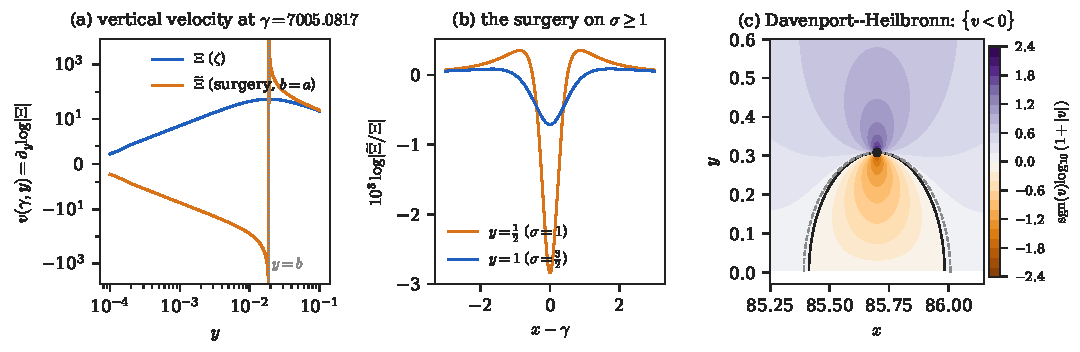
\includegraphics[width=\textwidth]{fig1_surgery.pdf}
\caption{(a) The vertical velocity $v=\partial_y\log|\Xi|$ on the line through the midpoint $\gamma=7005.0817$ of the Lehmer pair, for $\Xi$ and for the surgered function $\widetilde\Xi$ with $b=a=0.01885$; $v$ is positive for $\Xi$ and falls to $-\infty$ below the planted zero at $y=b$ for $\widetilde\Xi$. (b) The change $\log|\widetilde\Xi/\Xi|$ on $\Re s=1$ and $\Re s=\frac32$: at most $2.84\times10^{-3}$. (c) The downdraft of the Davenport--Heilbronn function below Spira's zero $85.6993+0.3085\,i$ (dot): colour gives $\operatorname{sgn}(v)\log_{10}(1+|v|)$, the solid curve is $v=0$, and the dashed curve is the half-disk of radius $0.3085$ of \cref{prop:pair}.}\label{fig:surgery}
\end{figure}

\section{Operator forms}\label{sec:operator}

An entire function $E$ is of Hermite--Biehler class if $|E(\bar z)|<|E(z)|$ for $z\in\C_+$; then $K_E(w,z)=(E(z)\overline{E(w)}-E^\#(z)\overline{E^\#(w)})/(2\pi i(\bar w-z))$, $E^\#(z)=\overline{E(\bar z)}$, is the reproducing kernel of a de Branges space \cite{deBrangesBook}.

\begin{proposition}[the Hermite--Biehler threshold]\label{prop:hb}
\Cref{mt:index}(i) holds.
\end{proposition}
\begin{proof}
By Hadamard's product for the even function $\Xi$ of order one (\cref{prop:pair}), which makes no assumption on the location of the zeros,
\[
\frac{|E_h(z)|^2}{|E_h(\bar z)|^2}=\prod_w\frac{|x-c_w+i(h+y-\delta_w)|^2}{|x-c_w+i(h-y-\delta_w)|^2},\qquad w=c_w+i\delta_w,
\]
with conjugate zeros grouped so that the product converges. A factor exceeds $1$ exactly when $(h+y-\delta_w)^2>(h-y-\delta_w)^2$, that is when $4y(h-\delta_w)>0$. If $h\ge\Theta=\sup\delta_w$, every factor is at least $1$ for $y>0$, and the factors with $\delta_w<0$, which exist, exceed $1$; so $E_h$ is of Hermite--Biehler class. If $h<\Theta$, some zero has $\delta_w>h$, and $E_h$ vanishes at $w-ih\in\C_+$, where $|E_h(\bar z)|<|E_h(z)|$ fails. $\Theta\le\frac12$ because $\zeta(s)\ne0$ for $\Re s\ge1$ \cite[Ch.~III]{Titchmarsh}.
\end{proof}

The threshold is due in substance to Lagarias \cite{Lagarias05}, whose theorem that the zeros of $\xi(s+h)\pm\xi(s-h)$ lie on the critical line for $|h|\ge\frac12$ rests on this Hermite--Biehler property, read in de Branges's theory.

\begin{proposition}[the current as a Hermite--Biehler defect]\label{prop:hbdefect}
\Cref{mt:index}(ii) holds.
\end{proposition}
\begin{proof}
$E_J^\#=\Xi-i\Xi'$ because $\Xi$ is real on $\R$. Expanding,
\[
E_J(z)\overline{E_J(w)}-E_J^\#(z)\overline{E_J^\#(w)}=2i\bigl[\Xi'(z)\overline{\Xi(w)}-\Xi(z)\overline{\Xi'(w)}\bigr],
\]
so $K_{E_J}(w,z)=(\Xi'(z)\overline{\Xi(w)}-\Xi(z)\overline{\Xi'(w)})/(\pi(\bar w-z))$. With $m=-\Xi'/\Xi$, $\Xi(z)N_m(z,w)\overline{\Xi(w)}=(-\Xi'(z)\overline{\Xi(w)}+\Xi(z)\overline{\Xi'(w)})/(z-\bar w)$, which is $\pi K_{E_J}(w,z)$. At $w=z$, $|E_J(z)|^2-|E_J(\bar z)|^2=2i\cdot2i\Im(\Xi'\bar\Xi)=4\Im(\Xi\bar\Xi')=-4\Im(\bar\Xi\Xi')=J$, since $J=2\partial_y|\Xi|^2=4\Re(\bar\Xi\,i\Xi')$. On $\R$ the difference quotient gives $\pi K(x,x)=\Xi'^2-\Xi\Xi''$.
\end{proof}

Given $J>0$ off $\mathcal U$ \cite{S01}, \cref{conj:1} holds if and only if $E_J$ is of Hermite--Biehler class. The number $\pi K_{E_J}(x,x)=\Xi'^2-\Xi\Xi''$ is the Laguerre expression, $\frac1{16}\int Q(p,x)p^2\dd p$ in the phase-space form of \cite{S01}.

\begin{theorem}[the index of the current]\label{thm:index}
The kernels $N_m$ on $\C_+$ minus the zeros of $\Xi$, and $K_{E_J}$ on $\C_+$, have exactly $N_+$ negative squares.
\end{theorem}
\begin{proof}
\emph{Lower bound.} Let $a_1,\dots,a_k$ be distinct zeros of $\Xi$ in $\C_+$ of multiplicities $\mu_j$. Near $a_j$, $m(z)=-\mu_j/(z-a_j)+O(1)$. For small $\varepsilon>0$ put $z_j=a_j-i\mu_j\varepsilon\in\C_+$, so that $m(z_j)=-i/\varepsilon+O(1)$. Then
\[
N_m(z_i,z_j)=\frac{-2i/\varepsilon+O(1)}{a_i-\bar a_j+O(\varepsilon)}=-\frac2\varepsilon\,\frac{i}{a_i-\bar a_j}+O(1).
\]
The matrix $C_{ij}=i/(a_i-\bar a_j)=\int_0^\infty e^{ia_it}\overline{e^{ia_jt}}\dd t$ is the Gram matrix of the linearly independent functions $e^{ia_jt}$ in $L^2(0,\infty)$, hence positive definite. So $[N_m(z_i,z_j)]$ has $k$ negative eigenvalues for small $\varepsilon$, and the number of negative squares is at least $\min(k,N_+)$ for every $k$.

\emph{Upper bound.} Let $N_+<\infty$ and let $P$ be the real even polynomial $\prod(1-z/w)$ over the non-real zeros $w$ with multiplicity. Then $\Xi_0=\Xi/P$ is even, real on $\R$, of order one with only real zeros, so $\Xi_0=\Xi_0(0)\prod_{c>0}(1-z^2/c^2)$ and $m_0=-\Xi_0'/\Xi_0=\sum_{c>0}\bigl[(c-z)^{-1}+(-c-z)^{-1}\bigr]$; each term $(c-z)^{-1}$, $c\in\R$, has the kernel $(c-z)^{-1}\overline{(c-w)^{-1}}\succeq0$, so $N_{m_0}\succeq0$. The remainder $-P'/P$ is $\sum_ah_a$ over the distinct zeros $a\in\C_+$ with $h_a(z)=\mu_a[(a-z)^{-1}+(\bar a-z)^{-1}]$, and a direct computation gives
\[
N_{h_a}(z,w)=\mu_a\bigl[f_a(z)\overline{f_{\bar a}(w)}+f_{\bar a}(z)\overline{f_a(w)}\bigr],\qquad f_a(z)=(a-z)^{-1},
\]
whose quadratic form $\mu_a\cdot2\Re(A\bar B)=\frac{\mu_a}2(|A+B|^2-|A-B|^2)$ has at most one negative square. Since the number of negative eigenvalues of a sum of Hermitian matrices is at most the sum of the numbers, $N_m=N_{m_0}+\sum_aN_{h_a}$ has at most $N_+$ negative squares.

\emph{From $N_m$ to $K_{E_J}$.} By \cref{prop:hbdefect}, on points where $\Xi\ne0$ the matrix of $\pi K_{E_J}$ is $DN D^*$ with $D=\operatorname{diag}(\Xi(z_i))$ invertible, which has the same inertia. $K_{E_J}$ is continuous on $\C_+\times\C_+$ and the zeros of $\Xi$ are isolated, so moving the points $z_i$ that are zeros slightly keeps every negative eigenvalue of $[K_{E_J}(z_i,z_j)]$ negative; hence the count on $\C_+$ equals the count on $\C_+$ minus the zeros.
\end{proof}

\Cref{thm:index} is \cref{mt:index}(iii) and \cref{mt:six}(b), since RH is $N_+=0$. Krein and Langer \cite{KL} proved that a function of the generalised Nevanlinna class $N_\kappa$ has at most $\kappa$ poles in $\C_+$; the theorem identifies the index of the current with the number $N_+$ of distinct zeros of $\Xi$ in $\C_+$. Bombieri \cite{Bombieri} proved the analogous count for Weil's form: if finitely many zeros fail RH, the number of negative eigenvalues of its truncations, for large truncations, is half the number of these zeros.

\begin{remark}[a self-adjoint operator for the zeros]\label{rem:hp}
If $N_+<\infty$ and $\Xi$ has no multiple real zero, $E_J$ has no real zeros and $K_{E_J}$ is the reproducing kernel of a Pontryagin space of entire functions of negative index $N_+$ \cite{KW}, which for $N_+=0$ is the de Branges space $\mathcal H(E_J)$ \cite{deBrangesBook}. Multiplication by $z$ in it is symmetric with deficiency indices $(1,1)$, and its self-adjoint extension associated with $A=\frac12(E_J+E_J^\#)=\Xi$ has the zeros of $\Xi$ as spectrum. A self-adjoint operator with the zeros of $\Xi$ as spectrum thus exists in a space with an indefinite metric of index $N_+$, and the metric is definite exactly under RH.
\end{remark}

\begin{corollary}\label{cor:shadowcount}
\Cref{mt:index}(iv) holds.
\end{corollary}
\begin{proof}
Where $\Xi\ne0$, $\Xi+it\Xi'=0$ if and only if $m(z)=-i/t$, and then $v=\Im m=-1/t<0$, so $J<0$; $\{J<0\}\subset\mathcal U$ by \cite{S01}. By \cref{prop:pair}, $v>0$ in $\C_+$ outside the finitely many half-disks over the zeros off the line, and $v\to0$ at the real axis away from real zeros; so for $t$ in a compact subset of $(0,\infty)$ the solutions of $m=-i/t$ lie in a fixed compact subset of $\C_+$ that contains no zero of $\Xi$ on its boundary. The zeros of $m+i/t=i(\Xi+it\Xi')/(t\Xi)$ in $\C_+$ therefore move continuously with $t$ and their number is constant on $(0,\infty)$. As $t\to0$, near each distinct zero $a$ of multiplicity $\mu$ there is exactly one solution, $z=a-i\mu t+O(t^2)$ (Rouch\'e's theorem for $-\mu/(z-a)+O(1)=-i/t$), and no other solution remains in the compact set. So the number is $N_+$.
\end{proof}

\begin{theorem}[shadow law]\label{thm:shadow}
\Cref{mt:index}(v) holds: under its hypotheses, with $\mu_0=u'(c)/u(c)\in\R$, $\Xi+it\Xi'$ has exactly one zero in $|z-c|<Cb^2$, at $c-\frac12\mu_0b^2+ib^2/2t+O(b^4)$, where $C$ and the implied constant depend only on $t$ and on bounds for $u'/u$ and its derivative on the disk.
\end{theorem}
\begin{proof}
With $\omega=z-c$, $m(z)=-2\omega/(\omega^2+b^2)-u'/u(z)$, and $u'/u(c+\omega)=\mu_0+O(\omega)$. For $|\omega|\le Cb^2$, $\omega^2+b^2=b^2(1+O(b^2))$, and $m=-i/t$ becomes $\omega=-\frac{b^2}2(\mu_0-i/t)+O(b^4)$. Rouch\'e's theorem on $|\omega|=Cb^2$ with $C>|\mu_0-i/t|$ gives exactly one solution.
\end{proof}

At the surgery of \cref{sec:surgery} at $7005.0817$ with $t=1$, the zero of $\widetilde\Xi+i\widetilde\Xi'$ lies at $7005.081715+2.000\times10^{-6}i$ for $b=0.002$, and its height divided by $b^2/2$ is $1.0000$, $1.0000$, $1.0004$, $1.0097$, $1.0895$ for $b=0.002,0.005,0.02,0.1,0.3$. The matrices $[N_m(z_i,z_j)]$ on $15$ points near the planted zero have exactly one negative eigenvalue, from $-3.6\times10^{-2}$ at $b=0.002$ to $-38.5$ at $b=0.3$, and on $12$ points near $\pm\gamma$ exactly two ($-1.2909$ twice at $b=0.02$), while for $\Xi$ itself the smallest eigenvalue is $+9.2\times10^{-10}$, at the level of the conditioning. For $\Xi_\epsilon$ and $\Xi_{\mathrm{DH}}$ the zeros of $F+iF'$ near the first off-line zeros are $9.64697122+0.29436266\,i$ and $85.74318239+0.05152712\,i$.

\subsection{De Branges's positivity condition}
De Branges \cite{deBranges86} proposed, for $E(z)=\xi(1-iz)$, the condition $\Re\langle F(z),F(z+i)\rangle_{\mathcal H(E)}\ge0$ for all $F$ with $F,F(\cdot+i)\in\mathcal H(E)$, which implies RH. Conrey and Li \cite{CL} derived from it the necessary condition $-\Re\{\xi'(\rho)\xi(1+\rho)\}\ge0$ at every zero $\rho$ and found the value $-5.389\times10^{-69}$ at the $34$-th zero in the normalisation $s(s-1)\pi^{-s/2}\Gamma(\frac s2)\zeta(s)$ of $\xi$.

\begin{theorem}\label{thm:debranges}
\Cref{mt:debranges}(i) holds.
\end{theorem}
\begin{proof}
Write $\xi=g\zeta$ and $Z(t)=e^{i\theta(t)}\zeta(\frac12+it)$. At $s=\frac12+it$, $\frac12s(s-1)=-\frac12(t^2+\frac14)$ and $\pi^{-s/2}\Gamma(\frac s2)=\pi^{-1/4}|\Gamma(\frac14+\frac{it}2)|e^{i\theta(t)}$, so $g(\frac12+it)=-|g|e^{i\theta(t)}$. Differentiating $\zeta(\frac12+it)=e^{-i\theta}Z$ at a zero gives $\zeta'(\rho)=-ie^{-i\theta(\gamma)}Z'(\gamma)$, hence $\xi'(\rho)=g(\rho)\zeta'(\rho)=i|g(\rho)|Z'(\gamma)$ and $-\Re\{\xi'(\rho)\xi(1+\rho)\}=|g(\rho)|Z'(\gamma)\Im\xi(\frac32+i\gamma)$. Moreover $\Xi'(\gamma)=i\xi'(\rho)=-|g|Z'(\gamma)$ and $\Xi(\gamma+i)=\xi(-\frac12+i\gamma)=\xi(\frac32-i\gamma)=\overline{\xi(\frac32+i\gamma)}$, which gives the second form. For the sign: if the zeros up to $\gamma_n$ are simple and on the line, $\operatorname{sgn}Z'(\gamma_n)=(-1)^{n+1}$ because $Z(0)=\zeta(\frac12)<0$. By Stirling's formula $\arg\Gamma(\sigma+i\tau)=\tau\log\tau-\tau+(\sigma-\frac12)\frac\pi2+O(1/\tau)$, so $\arg g(\frac32+it)=\theta(t)+\frac{5\pi}4+O(1/t)$ modulo $2\pi$. With $\theta(\gamma_n)=\pi(n-\frac32-S(\gamma_n))$ (the Riemann--von Mangoldt formula at the midpoint of the jump) and $a_n=\arg\zeta(\frac32+i\gamma_n)$, $\arg\xi(\frac32+i\gamma_n)=\pi n-\frac\pi4-\pi S(\gamma_n)+a_n+O(1/\gamma_n)$, so $\operatorname{sgn}\Im\xi(\frac32+i\gamma_n)=(-1)^{n+1}\operatorname{sgn}\sin(\frac\pi4+\pi S(\gamma_n)-a_n+O(1/\gamma_n))$, and the product with $\operatorname{sgn}Z'(\gamma_n)$ is the stated sign.
\end{proof}

Over the first $2469$ zeros, up to height $2999.5$, the condition fails at $252$ ($10.21\%$), first at $n=34$, $\rho=\frac12+111.0295355431697\,i$, where $-\Re\{\xi'(\rho)\xi(1+\rho)\}=-1.347\times10^{-69}=-5.389\times10^{-69}/4$, the value of Conrey and Li in our normalisation. The failure fraction in consecutive blocks of about $500$ zeros is $0.064$, $0.096$, $0.124$, $0.106$, $0.122$, and the sign of $\sin(\frac\pi4+\pi S(\gamma_n)-a_n)$ agrees with that of the condition at all but two of the $2469$ zeros. The standard deviation of $S(\gamma_n)$ over these zeros is $0.272$. We also reproduce $\Re\{\xi(1+282i)/\xi(2+282i)\}=-1.31957\times10^{-4}$ \cite{CL}.

\subsection{The Husimi current and the archimedean side}

\begin{theorem}\label{thm:husimi}
\Cref{mt:debranges}(ii) holds.
\end{theorem}
\begin{proof}
Let $W(a,k)=\frac1{2\pi}\int K(a+\frac q2)K(a-\frac q2)e^{-ikq}\dd q$ be the Wigner function of $K$. As in \cite[Prop.~11.1]{S01}, $H_F(k,y)=\frac\pi2\int W(a,k)\cosh(2ya)\dd a$ and $J_F(k,y)=2\pi\int W(a,k)\,a\sinh(2ya)\dd a$. Let $G$ be the centred Gaussian density on $\R^2$ with variances $\sigma_a^2=s/2$ in $a$ and $\sigma_k^2=1/2s$ in $k$, so that $\sigma_a\sigma_k=\frac12$. Then $W*G$ is the Husimi function of $K$, $(W*G)(a,k)=c\,|\langle\phi_{a,k},K\rangle|^2$ with $\phi_{a,k}$ the Gaussian wave packet of widths $(\sigma_a,\sigma_k)$ centred at $(a,k)$ and $c>0$ \cite{Cartwright}; it is real-analytic, nonnegative and vanishes only on a discrete set when $K\ne0$. For the nonnegative symbol $\sigma(a,k)=a\sinh(2ya)\,\delta(k-x)$,
\begin{align*}
0<\iint(W*G)\,\sigma&=\iint W\,(\sigma*G)\\
&=\sqrt{\frac s\pi}\,e^{y^2s}\int e^{-s(k-x)^2}\iint W(a,k)\bigl[a\sinh(2ya)+ys\cosh(2ya)\bigr]\dd a\dd k,
\end{align*}
because $\mathbb E[(a+g)\sinh(2y(a+g))]=e^{2y^2\sigma_a^2}(a\sinh(2ya)+2y\sigma_a^2\cosh(2ya))$ for $g\sim N(0,\sigma_a^2)$. The inner integral is $(J_F+4ysH_F)(k,y)/2\pi$.
\end{proof}

The inequality holds for every real even kernel, $\Phi_\epsilon$ included. At $x_0=9.45225$, $y=0.3$, $J_\epsilon=-1.031\times10^{-8}$ and $H_\epsilon=1.593\times10^{-9}$, so the pointwise quantity $J_\epsilon+4ysH_\epsilon$ is negative for $s<5.39$, while the Gaussian average of \cref{mt:debranges}(ii) is positive for every $s$ between $0.05$ and $500$ that we evaluated. The observable $\hat O_{x,y}$ of \cite{S01,S03} with Weyl symbol $a\sinh(2ya)\delta(k-x)\ge0$ is not a positive operator, since its expectation in the state $\Phi_\epsilon/\|\Phi_\epsilon\|$ is proportional to $J_\epsilon$, which is negative at $(x_0,0.3)$; its anti-Wick quantisation, the Gaussian average of \cref{thm:husimi}, is positive for every state.

\begin{proposition}\label{prop:arch}
\Cref{mt:debranges}(iii) holds. Moreover each Macdonald function $K_{ix}(2\pi Ne^p)$ of the expansion of $Q$ in \cite{S01} satisfies $-f''+(2\pi N)^2e^{2p}f=x^2f$, and for fixed $\alpha>0$ the function $x\mapsto K_{ix}(\alpha)$ has only real zeros.
\end{proposition}
\begin{proof}
At $s=\frac12+ix$, $\frac1s+\frac1{s-1}=2ix/(-x^2-\frac14)$ is purely imaginary, so $G(x,0)=\frac12\Re\psi(\frac14+\frac{ix}2)-\frac12\log\pi$, and $\theta'(x)=\frac{\dd}{\dd x}\Im\log\Gamma(\frac14+\frac{ix}2)-\frac12\log\pi$ is the same. The differential equation is Bessel's equation $z^2K''+zK'-(z^2-x^2)K=0$ in the variable $p=\log(z/2\pi N)$. The reality of the zeros is P\'olya's theorem \cite{Polya26}.
\end{proof}

By the Riemann--von Mangoldt formula $N(t)=\theta(t)/\pi+1+S(t)$, $\theta(t)/\pi+1$ is the smooth part of the counting function of the zeros, which Berry and Keating \cite{BerryKeating} obtained from the regularised Hamiltonian $xp$, and $\theta'/\pi$ is its density; off the zeros $v(x,0)=0$, so on the line the prime side also equals $\theta'(x)$, as $-\Re\,\zeta'/\zeta(\frac12+ix)=\theta'(x)$ shows directly. At the first zero, $G(\gamma_1,0)=\theta'(\gamma_1)=0.4052743722$.

\section{The heat flow}\label{sec:heat}

Let $\Phi_T(u)=e^{Tu^2/4}\Phi(u)$ and $\Xi_T(z)=\int_0^\infty\Phi_T(u)\cos(zu)\dd u$. In the normalisation of Polymath \cite{Polymath}, $\Xi_T(z)=8H_T(2z)$ with $H_t(z)=\int_0^\infty e^{tu^2}\Phi_{\mathrm P}(u)\cos(zu)\dd u$ \cite{S03}, so $\Lambda$ is the least $T$ with $\Xi_T$ real-rooted for all larger $T$, $0\le\Lambda\le0.2$ \cite{RT,PT}, and de Bruijn's theorem \cite{deBruijn,Polymath} reads: if the zeros of $\Xi_{T_0}$ satisfy $|\Im z|\le\Delta$, those of $\Xi_T$, $T\ge T_0$, satisfy $|\Im z|^2\le\max(\Delta^2-(T-T_0)/2,0)$. Differentiating under the integral, $\partial_T\Xi_T=-\frac14\Xi_T''$, and a simple zero moves with velocity $\dot z=\frac14\Xi_T''/\Xi_T'(z)=\frac12\sum_{z'\ne z}(z-z')^{-1}$. Put $\mathcal L_T=\Xi_T'^2-\Xi_T\Xi_T''$.

\begin{theorem}\label{thm:h1}
\begin{enumerate}[label=(\roman*)]
\item If $T>\Lambda$, then $\mathcal L_T>0$ on $\R$.
\item If $\Lambda>0$, then $\Xi_\Lambda$ has a real zero of multiplicity at least $2$.
\end{enumerate}
Hence \cref{mt:six}(c) holds.
\end{theorem}
\begin{proof}
(i) For $T>\Lambda$ the zeros of $\Xi_T$ are real and simple \cite[Cor.~1]{CSV}. $\Xi_T$ is even, and of order one in $z$, hence of order at most $\frac12$ in $z^2$, so $\Xi_T=\Xi_T(0)\prod_j(1-z^2/x_j^2)$ with $\Xi_T(0)>0$. Off the zeros, $\mathcal L_T=\Xi_T^2\cdot(-(\Xi_T'/\Xi_T)')=\Xi_T^2\sum_j[(x-x_j)^{-2}+(x+x_j)^{-2}]>0$, and at a simple zero $\mathcal L_T=\Xi_T'^2>0$.
(ii) Take $T_n\uparrow\Lambda$, $T_n>0$, and non-real zeros $z_n$ of $\Xi_{T_n}$. By de Bruijn's theorem $|\Im z_n|\le\frac12$, and by Theorem~1.5(i) of \cite{Polymath}, which makes the result of Ki, Kim and Lee \cite{KKL} uniform, the non-real zeros of $\Xi_T$ have $|\Re z|\le X(T_0)$ for $0<T_0\le T\le\frac12$; we take $T_0=\Lambda/2$ and $T_n\ge T_0$. A subsequence converges to some $z^*$. Since $\Xi_{T_n}\to\Xi_\Lambda$ locally uniformly and $\Xi_\Lambda$ is real-rooted, $z^*$ is real. By Hurwitz's theorem the two distinct zeros $z_n$, $\bar z_n$ converge to $z^*$, which is therefore a zero of multiplicity at least $2$.
For \cref{mt:six}(c): RH gives $\Lambda=0$ by \cite{RT}, and then (i) and \cite[Cor.~1]{CSV} give $\mathcal L_T>0$ and simple zeros for all $T>0$. If RH fails, $\Xi_0$ has a non-real zero, so $\Lambda>0$, $\Lambda\le0.2$ \cite{PT}, and by (ii) $\Xi_\Lambda$ has a multiple real zero $x^*$, where $\mathcal L_\Lambda(x^*)=0$. The formula for $\Lambda$ follows from (i), (ii) and \cite[Cor.~1]{CSV}.
\end{proof}

On $[0,40]$ the relative Laguerre margin $\min_x\mathcal L_T/(\Xi_T'^2+|\Xi_T\Xi_T''|)$ is $0.1741$, $0.1737$, $0.1732$, $0.1708$, $0.1685$, $0.1641$ at $T=0.2,0.1,0,-0.5,-1,-2$.

\begin{theorem}[Hermite local law]\label{thm:hermite}
\Cref{mt:heat}(i) holds.
\end{theorem}
\begin{proof}
Let $\tau=(T-T^*)/4$. For entire functions of order one, $\Xi_T=\sum_{k\ge0}(-\tau)^k\Xi_{T^*}^{(2k)}/k!$, the series converging locally uniformly (Cauchy's estimates with $\log\max_{|z|=r}|\Xi_{T^*}|=O(r\log r)$ give $|\Xi_{T^*}^{(2k)}|\le(Ck^{-1}\log k)^{2k}(2k)!$ on compact sets). Near $x^*$, $\Xi_{T^*}(x^*+\omega)=c\,\omega^m(1+O(\omega))$ with $c\ne0$ real. Since $e^{-t^2/2}e^{\omega t}=\sum\mathrm{He}_j(\omega)t^j/j!$, the operator $\sum_k(-\tau)^k\partial^{2k}/k!$ sends $\omega^m$ to $(2\tau)^{m/2}\mathrm{He}_m(\omega/\sqrt{2\tau})$, and $\omega^{m+j}$ to a polynomial of size $O(|\tau|^{(m+j)/2})$ for $\omega=O(|\tau|^{1/2})$. Hence $\Xi_T(x^*+\sqrt{2|\tau|}\,\eta)=c(2|\tau|)^{m/2}[\mathrm{He}_m^\pm(\eta)+O(|\tau|^{1/2})]$ uniformly for $\eta$ in compact sets, with $\mathrm{He}_m^+=\mathrm{He}_m$ for $\tau>0$ and $\mathrm{He}_m^-(\eta)=i^m\mathrm{He}_m(-i\eta)$ for $\tau<0$. The zeros of $\mathrm{He}_m$ are real and simple, and those of $\mathrm{He}_m^-$ are $i$ times them. Rouch\'e's theorem places exactly one zero of $\Xi_T$ near each, and by Hurwitz's theorem $\Xi_T$ has exactly $m$ zeros in a fixed small disk around $x^*$ for $T$ near $T^*$, so these are all of them. For $\tau>0$ each is simple and alone in a disk symmetric about $\R$; since $\Xi_T$ is real on $\R$, it is real. For $\tau<0$ only the zero near $\eta=0$ (present when $m$ is odd) can be real. Finally $2|\tau|=|T-T^*|/2$.
\end{proof}

\begin{theorem}[landing]\label{thm:landing}
\Cref{mt:heat}(ii) holds.
\end{theorem}
\begin{proof}
The zeros are $x_T\pm ib_T$ with $b_T^2=(T^*-T)/2(1+o(1))$ by \cref{thm:hermite} with $\mathrm{He}_2(\eta)=\eta^2-1$. Write $\Xi_T=q\,u$ near $x^*$ with $q=(z-x_T)^2+b_T^2$ and $u$ holomorphic, zero-free and real on $\R$, uniformly for $T$ near $T^*$. For real $x$, $\mathcal L[qu]=u^2\mathcal L[q]+q^2\mathcal L[u]$ and $\mathcal L[q]=2(x-x_T)^2-2b_T^2$, while $q^2=O(b_T^4)$ where $|x-x_T|\le2b_T$; so $\mathcal L_T<0$ exactly on an interval of half-width $b_T(1+O(b_T^2))$. For $z=x+iy$, $d=x-x_T$, $\partial_y\log|q|=2y(d^2+y^2-b_T^2)/|q|^2$ and $\partial_y\log|u|=\kappa_0y+O(y^3)$ with $\kappa_0$ bounded. Where $d^2+y^2\le4b_T^2$, $|q|^2\le81b_T^4$, so $v$ has the sign of $d^2+y^2-b_T^2+O(b_T^4)$. Where $4b_T^2\le d^2+y^2\le\delta_0^2$, with $\delta_0$ small and fixed, $d^2+y^2-b_T^2\ge\frac34(d^2+y^2)$ while $|q|^2\le2(d^2+y^2)^2$, so $v>0$ there. Hence near $x^*$ the boundary of $\{J_T<0\}$ is the circle $|z-x_T|=b_T$ displaced by $O(b_T^3)$.
\end{proof}

For $\Xi_\epsilon$ the first off-line pair lands at $T_c=0.747230705896$ at $x^*=8.993177745521$. At $T=0.745$ the set $\{\mathcal L_T<0\}$ has half-width $0.03338$ against $b_T=0.03339$ and $\sqrt{(T_c-T)/2}=0.03340$; for $T_c<T\le T_c+10^{-3}$ the two real zeros satisfy $\delta^2/(2(T-T_c))=1.0000$ ($10^{-5}$, $10^{-4}$) and $0.9998$ ($10^{-3}$), with $\delta$ their separation. Backwards, the Lehmer pairs collide at $T_c=-7.112047\times10^{-4}$ (gap $\delta_0=0.037698$ at $7005.08$) and $T_c=-6.241606\times10^{-4}$ ($\delta_0=0.035307$ at $17143.8$), close to $-\delta_0^2/2$ as the two-zero model of \cref{mt:heat}(ii) gives.

\begin{theorem}[two copies]\label{thm:twocopies}
\Cref{mt:heat}(iii) holds.
\end{theorem}
\begin{proof}
$H(x,y)=\frac14\iint\Phi(u)\Phi(v)e^{izu-i\bar zv}\dd u\dd v$ with $izu-i\bar zv=ix(u-v)-y(u+v)$ \cite{S01}. Write $\Phi=e^{-Tu^2/4}\Phi_T$ and $-T(u^2+v^2)/4=-T(u-v)^2/4-Tuv/2$. Since $e^{-T(u-v)^2/4}e^{ix(u-v)}=\mathbb E\,e^{i(x+g)(u-v)}$ for $g\sim N(0,T/2)$, $H(x,y)=\mathbb E\,\mathcal Z_T(x+g,y)$. Expanding $e^{-Tuv/2}=\sum_k(-T/2)^ku^kv^k/k!$, which is dominated because $\Phi_T$ decays doubly exponentially, and using $\frac12\int\Phi_T(u)(iu)^ke^{izu}\dd u=\Xi_T^{(k)}(z)$ gives the series. Differentiating in $y$ gives the statement for $J$.
\end{proof}

At $T=0.2$ the identity holds to $1.6\times10^{-15}$, $6.9\times10^{-12}$ and $2.6\times10^{-9}$ relative at $(5,0.05)$, $(14.1347,0.1)$ and $(21,0.3)$. In the language of \cite{S01}, the forward flow is a positive merge and the backward flow is not:

\begin{proposition}\label{prop:notmerge}
For $T>0$, $e^{Tu^2/4}=\mathbb E\,e^{ug}$ with $g\sim N(0,T/2)$, while $e^{-Tu^2/4}$ is not of the form $\int e^{ug}\mu(\dd g)$ for any positive measure $\mu$.
\end{proposition}
\begin{proof}
The first is the Gaussian moment generating function. By H\"older's inequality, $u\mapsto\log\int e^{ug}\mu(\dd g)$ is convex, while $-Tu^2/4$ is strictly concave.
\end{proof}

\begin{theorem}[three-state chains]\label{thm:spins}
\Cref{mt:heat}(iv) holds.
\end{theorem}
\begin{proof}
Let $S=\sum_iS_i$, $S_i\in\{-1,0,1\}$, with weight $e^{K\sum S_iS_{i+1}}$. Since $e^{TS^2/4}=\mathbb E\,e^{\sqrt{T/2}\,Sg}$ and $TS^2/4=\frac T4\sum_iS_i^2+\frac T2\sum_{i<j}S_iS_j$, $Z_{n,T}$ is the partition function of three-state spins with single-site weights $(e^{T/4},1,e^{T/4})$ and couplings $K\ge0$ (neighbours) and $T/2\ge0$ (all pairs). A spin with weights $(w,1,w)$ is the merged pair of two spins $\pm\frac12$ with coupling $e^{4\kappa_0\varsigma_1\varsigma_2}$, $w=e^{2\kappa_0}/2$ \cite{S01}; here $\kappa_0=\frac12\log2+T/8\ge0$. So $Z_{n,T}$ is the partition function of a spin-$\frac12$ ferromagnet, and its zeros lie on $|z|=1$ by the Lee--Yang theorem \cite{LeeYang,Griffiths69}. For $n=1$, $Z_{1,T}=e^{T/4}(z+z^{-1})+1$ vanishes where $z+z^{-1}=-e^{-T/4}$, which lies in $[-2,2]$ exactly when $T\ge-4\log2$. For $K=0$ and $n\ge2$, $Z_{n,0}=(z+1+z^{-1})^n$ has zeros of multiplicity $n$ at $e^{\pm2\pi i/3}$. On $|z|=1$, $z=e^{i\vartheta}$, $\partial_TZ_{n,T}=-\frac14\partial_\vartheta^2Z_{n,T}$, so \cref{thm:hermite} applies in $\vartheta$: for $T<0$ close to $0$ at most one of the $n$ zeros near $e^{2\pi i/3}$ is on the circle, and $\Lambda_n(0)=0$. For $n=2$, with $c=z+z^{-1}$, $Z_{2,T}=e^{T+K}(c^2-2)+2e^{T/4}c+1+2e^{-K}$, a quadratic in $c$ whose discriminant is $4q\,\Delta(q)$ with $q=e^{T/2}$ and
\[
\Delta(q)=2e^{2K}q^3-(e^K+2)q+1=(q-e^{-K})\bigl(2e^{2K}q^2+2e^Kq-e^K\bigr).
\]
For $K<\log4$ the positive root of the second factor is below $e^{-K}$, so $\Delta>0$ for $T>-2K$ and $\Delta<0$ for $T$ slightly below $-2K$. For $T\ge-2K$ the vertex $-e^{-3T/4-K}$ lies in $[-2,0)$ and the value at $c=-2$, $2e^{T+K}-4e^{T/4}+1+2e^{-K}$, is increasing in $T$ there and equals $(2e^{-K/2}-1)^2\ge0$ at $T=-2K$, while the value at $c=2$ is positive; so both roots $c$ lie in $[-2,2]$, which puts all four zeros on $|z|=1$. Hence $\Lambda_2(K)=-2K$. Finally, if $K>0$ and the $2n$ zeros of $Z_{n,0}$ on the circle are simple, they stay simple and, by the symmetry $z\mapsto1/\bar z$ of the zero set, on the circle for $T$ in a neighbourhood of $0$; so $\Lambda_n(K)<0$.
\end{proof}

\begin{table}[h]\centering\small
\begin{tabular}{@{}lccccc@{}}\toprule
$K$ & $n=2$ & $n=4$ & $n=8$ & $n=12$ & $n=16$\\\midrule
$0.1$ & $-0.2$ & $-0.05272$ & $-0.006991$ & $-0.001854$ & $-0.0006582$\\
$0.5$ & $-1.0$ & $-0.2445$ & $-0.04452$ & $-0.01231$ & $-0.004685$\\
$1$ & $-2.0$ & $-0.5063$ & $-0.09434$ & $-0.02965$ & $-0.01258$\\\bottomrule
\end{tabular}
\caption{$\Lambda_n(K)$ for chains of $n$ three-state spins, computed by bisection in $T$ with the zeros on $|z|=1$ counted by Sturm sequences. The column $n=2$ is $-2K$ exactly.}\label{tab:spins}
\end{table}

\section{Weil's functional and Li's coefficients}\label{sec:weil}

For a function $h$ holomorphic in a neighbourhood of the zeros, $W(h)=\sum_\rho h(\gamma_\rho)$ with $\rho=\frac12+i\gamma_\rho$ ($\gamma_\rho$ is complex when $\rho$ is off the line), summed with $\rho$ and $\bar\rho$ grouped.

\begin{theorem}[the Weil--Poisson form]\label{thm:weil}
Let $y>0$, $s=\frac12+y+ix$, $\xi(s)\ne0$, $h=h_{x,y}$ and $\varphi=\varphi_{x,y}$.
\begin{enumerate}[label=(\roman*)]
\item $J=4H\,W(h)$, $h=|\widehat\varphi|^2$ with $\widehat\varphi(r)=\int\varphi(u)e^{iru}\dd u=\sqrt y/(y+i(x-r))$, and $h=\widehat f$ for $f=\varphi*\tilde\varphi=\frac12e^{-y|u|}e^{-ixu}$, $\tilde\varphi(u)=\overline{\varphi(-u)}$.
\item For $y>\frac12$ Weil's explicit formula holds for $f$ with an absolutely convergent prime sum and is the ledger \eqref{eq:ledger}: the pole terms give $h(\frac i2)+h(-\frac i2)=\Re[\frac1s+\frac1{s-1}]$, the archimedean term gives $\frac12\Re\psi(\frac s2)-\frac12\log\pi$, and the prime term gives $A=\sum\Lambda(n)n^{-1/2-y}\cos(x\log n)$.
\item For $0<y\le\frac12$, $\sum\Lambda(n)n^{-1/2}|f(\log n)|=\infty$ and $h$ has poles at $x\pm iy$ in $|\Im r|\le\frac12$. The functions $\sum_{n\le X}\Lambda(n)n^{-s}-X^{1-s}/(1-s)$ converge to $-\zeta'/\zeta(s)$, whose real part is $A$, locally uniformly on $\{\Re s>\frac12+y_0\}$ if and only if $\Theta\le y_0$.
\end{enumerate}
\end{theorem}
\begin{proof}
(i) For a real zero $\gamma$, $h(\gamma)$ is the term $y/((x-\gamma)^2+y^2)$ of \cref{prop:pair}. For a pair $c\pm ib$, $h(r)=\frac1{2i}[(\bar z-r)^{-1}-(z-r)^{-1}]$ continues analytically, and $h(c+ib)+h(c-ib)=-\Im(z-c-ib)^{-1}-\Im(z-c+ib)^{-1}$, which is the pair term. The formulas for $\widehat\varphi$ and $f$ are direct integrations. (ii) Is the logarithmic derivative of the Hadamard product combined with $\xi'/\xi=\frac1s+\frac1{s-1}-\frac12\log\pi+\frac12\psi(\frac s2)+\zeta'/\zeta$, whose Dirichlet series converges absolutely for $\Re s>1$; the pole terms are computed from $h(r)=\frac12[(y+i(x-r))^{-1}+(y-i(x-r))^{-1}]$ at $r=\pm\frac i2$. (iii) The divergence is $\sum\Lambda(n)n^{-1/2-y}=\infty$ for $y\le\frac12$. Partial summation with $\psi(t)=t+E(t)$ gives $\sum_{n\le X}\Lambda(n)n^{-s}-X^{1-s}/(1-s)=-s/(1-s)+E(X)X^{-s}+s\int_1^XE(t)t^{-s-1}\dd t$, and $E(t)=O(t^{\frac12+\Theta+\epsilon})$ gives convergence to $-\zeta'/\zeta(s)$ for $\Re s>\frac12+\Theta$, locally uniformly. Conversely, a locally uniform limit on $\{\Re s>\frac12+y_0\}$ is holomorphic there and equals $-\zeta'/\zeta$ on $\Re s>1$, so $\zeta$ has no zero with $\beta>\frac12+y_0$.
\end{proof}

\Cref{thm:weil}(i) with \cite{S01} gives \cref{mt:six}(d): $\int Q\,p\sinh(yp)\dd p=16H\,W(h_{x,y})$, so \cref{conj:1} is Weil's positivity for the Poisson family $\varphi_{x,y}$, $(x,y)\in\mathcal U$. Indeed, under RH $\Xi$ has no zero in $\C_+$ and $W(h_{x,y})=J/4H>0$ there; conversely, if $\Xi$ has no zero in $\mathcal U$ and $W(h_{x,y})>0$ on $\mathcal U$, then $H>0$ and $J=4H\,W(h_{x,y})>0$ on $\mathcal U$, which is \cref{conj:1}. The zero side and $\Re\,\xi'/\xi$ agree to $3.3\times10^{-8}$ at twelve points with $0\le x\le1500$, $10^{-3}\le y\le0.4$, computed from the $2469$ zeros below $3000$ with a density tail, and to $6.9\times10^{-8}$ relative at the Lehmer pair near $7005$; the explicit formula at $(50,1.5)$ agrees to $2.9\times10^{-9}$.

\begin{theorem}[the Li--current identity]\label{thm:li}
With $w=1-1/s$,
\[
J=4H\,\Re\Bigl[\frac1{s(s-1)}\sum_{n\ge1}\lambda_nw^n\Bigr],
\]
the series converging absolutely for $|w|<R_\zeta=\min\bigl(1,\inf_{\beta>1/2}|1-1/\rho|\bigr)$. RH holds if and only if $R_\zeta=1$, and unconditionally $R_\zeta^2\ge1-1/T_0^2$ with $T_0=3\cdot10^{12}$.
\end{theorem}
\begin{proof}
With $F(w)=\log\xi(1/(1-w))$, $F'(w)=\sum_{n\ge0}\lambda_{n+1}w^n$ \cite{Keiper,BL}, and $F'(w)=s^2\,\xi'/\xi(s)$ for $s=1/(1-w)$, so $\xi'/\xi(s)=s^{-2}w^{-1}\sum\lambda_nw^n$ and $s^2w=s(s-1)$. The singularities of $F'$ in $|w|\le1$ are the points $1-1/\rho$ and $w=1$ ($s=\infty$), and $|1-1/\rho|<1$ exactly when $\beta>\frac12$. For $\beta>\frac12$, $|1-1/\rho|^2=1-(2\beta-1)/(\beta^2+\gamma^2)>1-1/\gamma^2$, and $|\gamma|>T_0$. At $s=\frac12+y+ix$, $|w|^2=1-2y/((y+\frac12)^2+x^2)<1$ for $y>0$.
\end{proof}

\Cref{thm:li} is \cref{mt:six}(e). On $\mathcal U$ the series needs about $|s|^2/y\approx10^{26}$ terms. It reproduces $\Re\,\xi'/\xi$ to ten digits at $(0,0.3)$, $(2,0.2)$, $(3,0.5)$ and $(\gamma_1,0.3)$ with the coefficients below.

\begin{lemma}[insensitivity of the Li coefficients]\label{lem:insens}
The estimate displayed in \cref{mt:li} holds.
\end{lemma}
\begin{proof}
Let $\phi(\beta)=n\log(1-1/(\beta+i\gamma))$ and $\Psi(b)=e^{\phi(\frac12+b)}+e^{\phi(\frac12-b)}$, the quantity in question being $\Psi(b)-\Psi(0)$ since $1-\bar\rho=\frac12-b+i\gamma$. $\Psi$ is even, so $|\Psi(b)-\Psi(0)|\le\frac{b^2}2\max_{|b'|\le b}|\Psi''(b')|$. Now $\phi'(\beta)=n/(\rho(\rho-1))$ with $|\rho(\rho-1)|\ge\gamma^2$, so $|\phi'|\le n/\gamma^2$; $\phi''=-n(2\rho-1)/(\rho(\rho-1))^2$, so $|\phi''|\le n(1+2\gamma)/\gamma^4\le3n/\gamma^3$; and $|1-1/\rho|^2=1-(2\beta-1)/(\beta^2+\gamma^2)\le1+2b/\gamma^2$, so $|e^\phi|\le e^{nb/\gamma^2}\le e^{1/2}$ for $n\le\gamma^2$. Hence $|\Psi''|\le2e^{1/2}(n^2\gamma^{-4}+3n\gamma^{-3})$.
\end{proof}

\begin{proof}[Proof of \cref{mt:li}]
$\lambda_n=\sum_\rho[1-(1-1/\rho)^n]$, with $\rho$ and $\bar\rho$ grouped. For $\rho_0=\frac12+i\gamma$, $1-1/\rho_0=e^{i\theta_\gamma}$ with $\theta_\gamma=2\arctan(1/2\gamma)$, so a conjugate pair on the line contributes $2(1-\cos n\theta_\gamma)\ge0$. Let $\lambda_n^{(0)}$ be the value obtained when every zero above $T_0=3\cdot10^{12}$ is moved onto the line with its ordinate kept; every term of $\lambda_n^{(0)}$ is nonnegative. By \cref{lem:insens} with $b<\frac12$, and since each quadruple off the line has two zeros with positive ordinate,
\[
|\lambda_n-\lambda_n^{(0)}|\le\frac{e^{1/2}}2\sum_{\gamma>T_0}\bigl(n^2\gamma^{-4}+3n\gamma^{-3}\bigr).
\]
Trudgian's bound $|N(t)-\frac t{2\pi}\log\frac t{2\pi e}-\frac78|\le0.112\log t+0.278\log\log t+2.51+0.2/t$ \cite{Trudgian} gives $N(t)\le\frac t{2\pi}\log t$ for $t\ge20$, and partial summation gives $\sum_{\gamma>T}\gamma^{-k}\le\frac k{2\pi(k-1)}(\log T+1)T^{1-k}$. With $T_0=3\cdot10^{12}$ this bounds the error by $1.93\times10^{-37}n^2+1.96\times10^{-24}n$, which is $2.2\times10^{-12}$ at $n=10^{12}$. For the main term keep one pair. If $5\le n\le10^{12}$, there is an ordinate $\gamma\in[n,3n]\subset(0,T_0]$: for $5\le n\le29$ one of $14.1347$, $21.0220$, $30.4249$ lies there, and for $n\ge30$ Trudgian's bound gives $N(3n)-N(n)\ge\bar N(3n)-\bar N(n)-E(3n)-E(n)$, with $\bar N(t)=\frac t{2\pi}\log\frac t{2\pi e}+\frac78$ and $E(t)$ the right side of Trudgian's bound; this lower bound is $14.4$ at $n=30$ and increasing in $n$, since for $n\ge30$ the derivative of $\bar N(3n)-\bar N(n)$ exceeds $1$ while that of $E(3n)+E(n)$ is below $0.02$. Then $n\theta_\gamma\in[2n\arctan\frac1{6n},2n\arctan\frac1{2n}]\subset[0.3332,1]$, so $\lambda_n^{(0)}\ge2(1-\cos0.3332)=0.1099$. For $n\le4$ the first zero gives $n\theta_{\gamma_1}\in[0.0707,0.283]$ and $\lambda_n^{(0)}\ge2(1-\cos0.0707)=0.0049$.
\end{proof}

\paragraph{Computed coefficients.} By a Cauchy integral of $F'$ on $|w|=0.9998$ with $2^{18}$ nodes, which uses no zeros, $\lambda_n>0$ for $n\le30000$, with minimum $\lambda_1=0.0230957090$ (exactly $1+\frac{\gamma_E}2-\frac12\log4\pi=0.02309570896612$), $\lambda_2=0.0923457352$, $\lambda_3=0.2076389206$, $\lambda_{100}=118.6038$, $\lambda_{1000}=2326.0532$ and $\lambda_{30000}=120740.3$, against Keiper's asymptotic $\frac n2(\log\frac n{2\pi}-1+\gamma_E)=120724.4$ \cite{Keiper}. For $n\le1200$ a second integral on $|w|=0.99$ with $8192$ nodes agrees to $2.3\times10^{-8}$, and the sum over the zeros below $3000$ with a density tail agrees within its error bound.

\paragraph{Windows.} Weil's functional restricted to test functions of bounded support was studied by Bombieri \cite{Bombieri}. For a finite-dimensional space $V$ of real functions supported in $[-L/2,L/2]$ let
\[
\mu(V)=\min_{0\ne g\in V}\frac{W(\widehat{g*\tilde g})}{\|g\|_2^2},\qquad W(\widehat{g*\tilde g})=\frac1\pi\int_\R\widehat g(t-i\delta)\overline{\widehat g(t+i\delta)}\,\frac{\xi'}\xi(c+it)\dd t,\quad\delta=c-\tfrac12,
\]
the contour integral holding for every $c>\frac12+\Theta$ by the argument principle and the functional equation. A negative $\mu(V)$ shows that Weil's form is not positive on windows of length $L$. We use the spaces $V_h(L)$ of cubic B-splines with knot spacing at most $h$, and $V_h(L,T_0)$ spanned by $B_j(u)\cos(T_0u)$ and $B_j(u)\sin(T_0u)$. For $\zeta$ on $V_{0.1}(L)$, with $c=1.5$ and $c=2.6$ agreeing and agreeing with the zero sum, $\mu=0.312$, $9.57\times10^{-3}$, $2.32\times10^{-5}$, $1.51\times10^{-9}$, $3.13\times10^{-11}$, $2.68\times10^{-12}$, $7.9\times10^{-13}$ at $L=0.3$, $0.69$, $1$, $2$, $3$, $4$, $5$. Connes and Consani proved positivity at the archimedean place for $g$ supported in $[2^{-1/2},2^{1/2}]$ multiplicatively \cite{CC}, that is, $L=\log2$ here.

\section{The merge}\label{sec:merge}

\begin{theorem}[truncations]\label{thm:trunc}
\Cref{mt:merge}(i) holds.
\end{theorem}
\begin{proof}
Let $\phi_n$ be the $n$-th term of \eqref{eq:Phi} and $\mathcal T=\Phi-\Phi^\flat$ the omitted part, a sum of $\phi_n$ with $n\ge2$. Then $\phi_n'(0)=4e^{-\pi n^2}(-4\pi^3n^6+15\pi^2n^4-7.5\pi n^2)<0$ for $n\ge2$, so $\mathcal T'(0)<0$. For the Epstein kernel each term is $2a(a-2)e^{u/2-a}$, $a=c_0Qe^u$, $c_0=\pi/\sqrt6$, with derivative $2a(-a^2+4.5a-3)e^{-a}$ at $u=0$, negative for $a>3.69$; the omitted forms have $Q\ge3$, $a\ge3c_0=3.85$. Integrating by parts twice, $\int_0^\infty\mathcal T(u)\cos(xu)\dd u=-\mathcal T'(0)/x^2+o(x^{-2})$, while $\Xi(x)$ and $\Xi_\epsilon(x)$ decay exponentially. So $F(x)=\mathcal T'(0)x^{-2}(1+o(1))<0$ for large $x$, and $F$, which is analytic, has finitely many real zeros. Each term of $\Phi^\flat$ is positive for $u\ge0$, and restricting to $u\in[U,U+1]$ with $2\pi e^{2U}=y$ in $F(iy)=\int_0^\infty\Phi^\flat\cosh(yu)\dd u$ gives $\log F(iy)\ge\frac y2\log y-O(y)$. So $F$ is entire of order one and infinite type, hence has infinitely many zeros by Hadamard's theorem, all but finitely many of them non-real.
\end{proof}

The real zeros of the truncations at $N=1,2,3,4$ number $1$, $7$, $15$, $31$, the last at $14.044$, $39.532$, $65.03$, $103.37$, and each truncation has non-real zeros with real part below $130$ ($3$, $4$, $6$, $7$ in $\Im z<12$). The heights are close to $4(N+1)^2$, where $e^{-\pi x/4}$ and $e^{-\pi(N+1)^2}$ balance. The $3$-smooth and $5$-smooth truncations have the same $25$ and $43$ real zeros as $\Xi$ below $90$ and $130$, since their omitted tails start at $n=5$ and $n=7$. The Epstein truncations with $V=20$ and $30$ reproduce the real zeros $5.131$, $12.075$, $15.063$ of $\Xi_\epsilon$ and its off-line zero near $9.452+0.660\,i$.

\begin{proposition}[evenness]\label{prop:even}
\Cref{mt:merge}(ii) holds. Consequently a kernel whose cosine transform has infinitely many real zeros has all odd derivatives zero at $0$.
\end{proposition}
\begin{proof}
Repeated integration by parts gives $\int_0^\infty f\cos(xu)\dd u=\sum_{j<k_0}(-1)^{j+1}f^{(2j+1)}(0)x^{-2j-2}+O(x^{-2k_0-2})$ for every $k_0$. If $k$ is the least index with $f^{(2k+1)}(0)\ne0$, the transform is $(-1)^{k+1}f^{(2k+1)}(0)x^{-2k-2}(1+O(x^{-2}))\ne0$ for large $|x|$. It is analytic in $|\Im z|<c$, so it has finitely many zeros in every compact interval.
\end{proof}

\begin{theorem}[no cosh factor]\label{thm:cosh}
\Cref{mt:merge}(iii) holds. Evaluated with $4000$ terms of \eqref{eq:Phi} on a grid of step $5\times10^{-5}$, $\Phi(iy)$ is real, positive on $[0,y^*)$, has a single zero $y^*=0.638830$ in $(0,0.7739]$, where it changes sign, and is negative on $(y^*,0.7739]$, its smallest absolute value on the grid there, $1.6\times10^{-7}$, being at the right end; so the hypothesis holds for every $a\ge2.03$ except $a^*=\pi/2y^*=2.45886$.
\end{theorem}
\begin{proof}
$\Phi$ is analytic and doubly-exponentially decaying in $|\Im u|<\pi/4$. For $a>2$ the first pole of $\operatorname{sech}(au)$ above $\R$ is $i\pi/2a$, inside this strip, with residue $-i/a$. Shifting $\int_\R\Phi(u)\operatorname{sech}(au)e^{ixu}\dd u$ to $\Im u=c_a\in(\pi/2a,\min(3\pi/2a,\pi/4))$ gives $2\pi i\cdot(-i/a)\Phi(i\pi/2a)e^{-\pi x/2a}+O(e^{-c_ax})$, and half of it is the cosine integral. If $\Phi(i\pi/2a)\ne0$, the transform $F_a$ of the even, positive, doubly-exponentially decaying kernel $\Phi\operatorname{sech}(au)$ has no real zeros for large $|x|$ and, as in \cref{thm:trunc}, infinitely many zeros; so it is not in the Laguerre--P\'olya class. If $\Phi=\cosh(au)\Phi_0$, then $\Phi_0=\Phi\operatorname{sech}(au)$.
\end{proof}

Multiplying a kernel by $\cosh(au)$ preserves the reality of the zeros of its transform, since $\int\cosh(au)\Phi_0(u)\cos(zu)\dd u=\frac12[F_0(z+ia)+F_0(z-ia)]$ \cite{deBruijn}; \cref{thm:cosh} shows that $\Phi$ has no such factor with $a>2$, $a\ne a^*$. At $x=30$ the ratio of $F_a$ to its leading term is $1.0112$, $1.0005$, $1.00004$ for $a=3,4,6$. For $a=0.5,1,1.5,2,2.5$ the transform $F_a$ has $6,6,3,1,0$ real zeros in $(0,40)$ and $0,0,1,2,3$ zeros in $(0,40)\times(0,4)$, against $6$ and $0$ for $\Xi$.

\begin{theorem}[the $\nu$-flow]\label{thm:nuflow}
\Cref{mt:merge}(iv) holds.
\end{theorem}
\begin{proof}
For $\Re s<0$, $\mathbb E[X^{s/2}]=\Gamma(-\frac s2)^{-1}\int_0^\infty\beta^{-s/2-1}\mathbb E\,e^{-\beta X}\dd\beta$ with $\mathbb E\,e^{-\beta S_\nu}=(x/\sinh x)^\nu$, $x=\sqrt{2\beta}$ \cite{S01}. Expanding $(x/\sinh x)^\nu=(2x)^\nu\sum_kc_k(\nu)e^{-(\nu+2k)x}$, $c_k(\nu)=\Gamma(k+\nu)/(\Gamma(\nu)k!)$, and integrating term by term,
\[
M_\nu(s)=\Bigl(\frac\pi2\Bigr)^{s/2}\frac{2^{1+s/2+\nu}\,\Gamma(\nu-s)}{\Gamma(-s/2)}\,D_\nu(\nu-s),\qquad D_\nu(w)=\sum_{k\ge0}c_k(\nu)(\nu+2k)^{-w},
\]
first for $\Re s<0$ and then by continuation. At $\nu=2$, $c_k=k+1$ and $D_2(w)=2^{-w}\zeta(w-1)$, and the duplication formula recovers $M_2=2\xi$. Since $\partial_\nu c_k|_{\nu=2}=(k+1)(\mathsf H_{k+1}-1)$ and $\partial_\nu(\nu+2k)^{-w}=-w(\nu+2k)^{-w-1}$,
\[
\partial_\nu D_\nu(w)\big|_{\nu=2}=2^{-w}\bigl[E(w-1)-\zeta(w-1)-\tfrac w2\zeta(w)\bigr],\quad E(s)=\sum_n\mathsf H_nn^{-s}=-\zeta'(s)+\gamma_E\zeta(s)+\Upsilon(s).
\]
At a zero $\rho$ of $\xi$, $D_2(2-\rho)=0$ because $\zeta(1-\rho)=0$. Writing $M_\nu(s)=A_\nu(s)D_\nu(\nu-s)$ and differentiating, $\dd\rho/\dd\nu=-\partial_\nu M/\partial_sM=1+\partial_\nu D(2-\rho)/D_2'(2-\rho)$, with $D_2'(2-\rho)=2^{\rho-2}\zeta'(1-\rho)\ne0$ for a simple zero. Substituting gives the formula. The implicit function theorem applies because $\partial_sM_2(\rho)=2\xi'(\rho)\ne0$.
\end{proof}

The formula agrees with finite differences of $\log M_\nu$ in $\nu$ to eight digits at $s=0.3+5i$, $-0.4+3i$ and $0.7+9i$. For the first ten zeros $\Re\,\dd\rho/\dd\nu=-0.567$, $+0.162$, $-0.982$, $+1.527$, $-2.162$, $+0.710$, $+0.862$, $-2.753$, $+4.174$, $-3.281$; at $\gamma_1$ it matches the slope $(0.443-0.556)/0.2=-0.565$ of the zero path of \cite{S01}. Of the $1517$ zeros with $10<\gamma<2000$, $761$ ($50.2\%$) move to the right as $\nu$ increases through $2$. The members of each Lehmer pair move in opposite directions: $+6078$ and $-6644$ at $7005.06$, $7005.10$, and $+23371$ and $-23088$ at $17143.79$, $17143.82$. So near $\nu=2$ the zeros of $M_\nu$ lie on both sides of the line, and the line is reached from both sides.

\begin{theorem}[Hausdorff moments]\label{thm:hausdorff}
\Cref{mt:six}(f) holds.
\end{theorem}
\begin{proof}
$\log\Xi(z)=\log\Xi(0)-\sum_{m\ge1}S_mz^{2m}/m$ for $|z|<|w_1|$, from the product over the zeros with $\Re w>0$; zeros come in pairs $w,\bar w$, so $S_m$ is real. With $Z(h)=\Xi(-ih)=\frac12\int\Phi(u)e^{hu}\dd u$, the partition function of Riemann's spin \cite{Newman76,S01}, the cumulants are $\kappa_{2m}=(-1)^{m+1}(2m)!S_m/m$. If RH holds, $S_{m+1}=\sum_\gamma\gamma^{-2}(\gamma^{-2})^m=\int_0^1a^m\nu(\dd a)$ with the finite positive measure $\nu=\sum_{\gamma>0}\gamma^{-2}\delta_{\gamma^{-2}}$ on $[0,\gamma_1^{-2}]$. Conversely, if $S_{m+1}=\int_0^1a^m\nu(\dd a)$, then $\sum_mS_{m+1}x^m=\int\nu(\dd a)/(1-xa)$ is holomorphic off $[1,\infty)$; but it equals $\sum_{\Re w>0}(w^2-x)^{-1}$ near $0$, a meromorphic function with a pole at each distinct $w^2$. So every $w^2$ lies in $[1,\infty)$ and every zero is real. Unconditionally, the zeros with $|\Re w|\le3\cdot10^{12}$ are real, and the others contribute at most $2\sum_{|w|>3\cdot10^{12}}|w|^{-2m}<\gamma_1^{-2m}$ in absolute value, so $S_m\ge\gamma_1^{-2m}-2\sum_{|w|>3\cdot10^{12}}|w|^{-2m}>0$.
\end{proof}

By Hausdorff's theorem \cite{Hausdorff} the moment property is the complete monotonicity $\sum_{j=0}^k(-1)^j\binom kjS_{m+j+1}\ge0$ for all $k,m\ge0$, an explicit family of inequalities for the cumulants. The Hankel determinants of $s_m=\gamma_1^{2m}S_m$, computed from the Taylor coefficients of $\log\Xi$ by a discrete Cauchy integral, are $\det[s_{i+j+1}]_{i,j<k}=4.62$, $3.11$, $0.110$, $7.59\times10^{-5}$, $6.41\times10^{-10}$ and $\det[s_{i+j+2}]_{i,j<k}=1.48$, $0.246$, $1.26\times10^{-3}$, $9.49\times10^{-8}$, $8.18\times10^{-14}$ for $k=1,\dots,5$, all positive.

\begin{proof}[Proof of \cref{mt:six}]
Parts (a)--(f) are \cref{thm:jensen}, \cref{thm:index}, \cref{thm:h1}, \cref{thm:weil}, \cref{thm:li} and \cref{thm:hausdorff}. Each is equivalent to RH, which is equivalent to \cref{conj:1} by \cite{S01}.
\end{proof}

\section{The primes as generators}\label{sec:primes}

\begin{theorem}\label{thm:gen}
\Cref{mt:primes}(i) holds.
\end{theorem}
\begin{proof}
By induction, $\langle G_k\rangle$ is the set of $\ell_k$-smooth integers: every $n\in[2,\ell_{k+1})$ has all its prime factors at most $\ell_k$, and $\ell_{k+1}$ has not, so $g_{k+1}=\ell_{k+1}$. An atom of $(\mathbb Z_{\ge1},\cdot)$, an element $\ne1$ that is not a product of two elements $\ne1$, lies in every generating set, and every non-atom $>1$ is a product of smaller elements; the atoms are the primes. In Hilbert's monoid $\{n\equiv1\bmod4\}$ the atoms $9,21,49$ satisfy $441=9\cdot49=21\cdot21$, so the minimal generating set exists and factorisation is not unique; its Dirichlet series $\sum_{n\equiv1(4)}n^{-s}=\frac12[(1-2^{-s})\zeta(s)+L(s,\chi_{-4})]$ is a sum of two Euler products, the shape of the Davenport--Heilbronn function. Uniqueness in $\mathbb Z$ comes from Euclid's lemma, an additive fact.
\end{proof}

\begin{lemma}[the triad's digits]\label{lem:digits}
\Cref{mt:primes}(ii) holds. Moreover $n\equiv\pm1\pmod6$ if and only if $n$ is odd and $3\nmid n$, and then the sign is $\chi_{-3}(n)$.
\end{lemma}
\begin{proof}
Write $n=3^vm$, $3\nmid m$. The balanced-ternary expansion of $n$ is that of $m$ shifted by $v$ places, and the last digit $d\in\{\pm1\}$ of $m$ satisfies $m\equiv d\pmod3$, so $d=\chi_{-3}(m)$; complete multiplicativity follows, and $\sum_nd(n)n^{-s}=\sum_v3^{-vs}\sum_{3\nmid m}\chi_{-3}(m)m^{-s}$. Since $3^i\equiv1\pmod2$, $s_3(n)\equiv n\pmod2$, and $\sum(-1)^nn^{-s}=-\eta(s)$. The last statement is the Chinese remainder theorem.
\end{proof}

With $L_\pm(x)=\sum_{n\le x,\,n\equiv\pm1(6)}\lambda(n)$, the Euler products give $\sum_{(n,6)=1}\lambda(n)n^{-s}=(1+2^{-s})(1+3^{-s})\zeta(2s)/\zeta(s)$ and $\sum_{(n,6)=1}\lambda(n)\chi_{-3}(n)n^{-s}=(1-2^{-s})(1-3^{-2s})\zeta(2s)/L(s,\chi_{-3})$; as for \cite[Prop.~3.1]{S01}, RH is equivalent to $L_++L_-=O(x^{1/2+\varepsilon})$, and the Riemann Hypothesis for $L(s,\chi_{-3})$ to $L_+-L_-=O(x^{1/2+\varepsilon})$. The terms of the poles at $s=\frac12$ are $-1.8439\sqrt x$ and $+0.4061\sqrt x$, and the logarithmic means of $(L_+\pm L_-)/\sqrt x$ over $[10^4,10^{10}]$ are $-1.8383$ and $+0.4077$.

\begin{proposition}[the observer-induction barrier]\label{prop:barrier}
\Cref{mt:primes}(iii) holds: for signs $\varepsilon=(\varepsilon_\ell)$ put $M_\varepsilon(x,k)=\sum\mu^2(n)\prod_{\ell\mid n}\varepsilon_\ell$ over the $\ell_k$-smooth $n\le x$. Then $M_\varepsilon(x,k)=M_\varepsilon(x,k-1)+\varepsilon_{\ell_k}M_\varepsilon(x/\ell_k,k-1)$, the bound $B(x,k)=B(x,k-1)+B(x/\ell_k,k-1)$, $B(x,0)=\mathbf 1_{x\ge1}$, that the triangle inequality gives is the number $Q_k(x)$ of squarefree $\ell_k$-smooth $n\le x$, and $\max_\varepsilon|M_\varepsilon(x,k)|=Q_k(x)$. For every $\sigma\ge0$, $Q_k(x)\le x^\sigma\prod_{i\le k}(1+\ell_i^{-\sigma})$, and the product is bounded in $k$ exactly when $\sigma>1$.
\end{proposition}
\begin{proof}
Split the squarefree $\ell_k$-smooth $n$ by whether $\ell_k\mid n$. The recursion for $B$ counts the same set, and $\varepsilon\equiv+1$ attains it; $M(x)$ is the case $\varepsilon\equiv-1$ with $k=\pi(x)$. Rankin's bound is $Q_k(x)\le\sum_n(x/n)^\sigma$ over squarefree $\ell_k$-smooth $n$, and $\prod(1+\ell^{-\sigma})$ converges exactly for $\sigma>1$.
\end{proof}

\begin{proposition}[the observer path]\label{prop:path}
\Cref{mt:primes}(iv) holds. More generally, for $y\ge\sqrt x$, $M(x,y)=M(x)+\sum_{m\le x/y}\mu(m)(\pi(x/m)-\pi(y))$, and for $1<u\le2$, $L(x,x^{1/u})=\sum_{n\le x,\,P^+(n)\le x^{1/u}}\lambda(n)=-\zeta(2)x/\log^2x+O_u(x/\log^3x)$.
\end{proposition}
\begin{proof}
If $n\le x$ has a prime factor $\ell>y\ge\sqrt x$, then $n=\ell m$ with $m\le x/y<\ell$ and $\mu(n)=-\mu(m)$, which gives the identity, and $y=x/2$ leaves only $m=1$. Put $z=x^{1-1/u}\le y$ and $\mathcal L=\log x$. By the prime number theorem with the classical error term \cite[Ch.~III]{Titchmarsh}, $M(t),L(t)\ll t\,e^{-c\sqrt{\log t}}$ and $\pi(t)=\operatorname{li}(t)+O(te^{-c\sqrt{\log t}})$; since $\log(x/m)\ge\mathcal L/u$ for $m\le z$, the errors, $M(x)$ and $\pi(y)M(z)$ contribute $O(xe^{-c'\sqrt{\mathcal L}})$. Write $\operatorname{li}(x/m)=\frac xm[(\mathcal L-\log m)^{-1}+(\mathcal L-\log m)^{-2}+O(\mathcal L^{-3})]$ and expand in powers of $\log m/\mathcal L$ up to order $3$; the remainders are controlled by partial summation against $M(t)$, and the sums $\sum_{m\le z}\mu(m)(\log m)^j/m$ equal $0,-1,-2\gamma_E$ for $j=0,1,2$ up to $O(e^{-c\sqrt{\log z}})$, from $1/\zeta(1+w)=w-\gamma_Ew^2+O(w^3)$. Collecting terms, $\sum_{m\le z}\mu(m)\operatorname{li}(x/m)=x[-\mathcal L^{-2}-2\gamma_E\mathcal L^{-3}-2\mathcal L^{-3}]+O(x\mathcal L^{-4})$. For $L$ the same argument with $\zeta(2+2w)/\zeta(1+w)=\zeta(2)w+O(w^2)$ gives the leading term.
\end{proof}

\paragraph{The record to $10^{10}$.} An exact segmented sieve over all $n\le10^{10}$, in integer arithmetic, gives $\pi(10^{10})=455{,}052{,}511$, $M(10^{10})=-33{,}722$ and $L(10^{10})=-116{,}026$, in agreement with the published values \cite{OEISpi,OEISM,OEISL}, and the first $x>1$ with $L(x)>0$ at $906{,}150{,}257$ \cite{Tanaka}. $L(x)>0$ at $305{,}426$ integers $x\le10^{10}$ and $M$ changes sign $131{,}477$ times. On $[10^4,10^{10}]$: $(\psi(x)-x)/\sqrt x\in[-0.751,0.791]$; $(\pi(x)-\operatorname{li}(x))\log x/\sqrt x\in[-2.447,-0.421]$; $M(x)/\sqrt x\in[-0.464,0.571]$; $L(x)/\sqrt x\in[-1.3583,0.0275]$. Schoenfeld's bound $|\psi(x)-x|<\sqrt x\log^2x/8\pi$ for $x\ge73.2$, which holds under RH \cite{Schoenfeld}, is met with ratio at most $0.918$ (as $x\uparrow97$), and at most $0.0396$ on $[10^9,10^{10}]$. At $x=10^{10}$ the observer path gives $M(x,\sqrt x)=-21{,}940{,}269=-219.40\sqrt x$, against $-214.45\sqrt x$ from \cref{prop:path}; $L(x,\sqrt x)=-373.17\sqrt x$; $M(x,x^{2/3})=-212.98\sqrt x$; $M(x,x/2)=220{,}064{,}566=2200.6\sqrt x$; and $M(x)=-0.337\sqrt x$. The balance at the scale $\sqrt x$ is reached only when the last primes, those in $(x/2,x]$, are added, and their number is $\pi(x)-\pi(x/2)$.

\paragraph{Beurling systems.} Generalised prime systems in the sense of Beurling are generated freely by their primes, so \cref{mt:primes}(i) holds for them by construction. Hilberdink \cite{Hilberdink} proved that if $N_{\mathrm B}(x)=ax+O(x^{\beta+\varepsilon})$ and $\psi_{\mathrm B}(x)=x+O(x^{\alpha+\varepsilon})$ then $\max(\alpha,\beta)\ge\frac12$, and Broucke, Debruyne and R\'ev\'esz \cite{BDR} constructed, for every $\alpha\in[0,1)$ and $\beta\in[\frac12,1)$, a system for which these are the optimal exponents. So the generating rule, together with the regularity of the integers at the square-root scale, does not force $\alpha=\frac12$; for $\mathbb Z$ the statement $\alpha=\frac12$ is RH.

\section{The comparison functions}\label{sec:compare}

\begin{proposition}[shared structure]\label{prop:shared}
Let $F\in\{\Xi,\Xi_\epsilon,\Xi_{\mathrm{DH}}\}$. Then $F$ is even, entire of order one, real on $\R$, with $F(s)=F(1-s)$ in the variable $s=\frac12+iz$, and its zeros lie in a horizontal strip. For each such $F$: the pair formula (\cref{prop:pair}); \cref{thm:downdraft}; the Jensen--Riesz formula of \cref{thm:jensen} with $Y$ above the strip; the identities of \cref{prop:hbdefect}, the index formula of \cref{thm:index} and the count of \cref{cor:shadowcount} (whose inclusion in $\mathcal U$ is specific to $\zeta$); the shadow law (\cref{thm:shadow}); and the Hermite and landing laws of \cref{thm:hermite,thm:landing} for its heat flow. For $F\in\{\Xi,\Xi_\epsilon\}$, which are transforms of positive even doubly-exponentially decaying kernels, also the Husimi inequality (\cref{thm:husimi}) and the Macdonald expansion with tail positivity of the Wigner function \cite{S01}. $\Xi_\epsilon$ and $\Xi_{\mathrm{DH}}$ have zeros off the real axis. Hence no conjunction of these properties implies that the zeros are real.
\end{proposition}
\begin{proof}
The proofs cited use only the stated properties; the strip for $\Xi_\epsilon$ is \cref{prop:sepproved}(ii), and for $\Xi_{\mathrm{DH}}$, $|f(s)-1|\le\sum_{n\ge2}n^{-\sigma}<1$ for $\sigma\ge\frac52$, so its zeros have $|\Im z|<2$. The off-line zeros are $s_0$ and Spira's zeros \cite{S01,Spira}.
\end{proof}

\begin{proposition}[shared inequalities, computed]\label{prop:sharedcomp}
The following hold for $\zeta$ (the cited theorems) and, as computed, for $Z_\epsilon$.
\begin{enumerate}[label=(\roman*)]
\item The Tur\'an inequalities $b_k^2>\frac{2k-1}{2k+1}b_{k-1}b_{k+1}$ for the moments $b_k=\int_0^\infty\Phi(u)u^{2k}\dd u$, proved for all $k$ for $\Phi$ by Csordas, Norfolk and Varga \cite{CNV}; for $\Phi_\epsilon$ for $k\le69$, with minimum margin $1-\frac{2k-1}{2k+1}b_{k-1}b_{k+1}/b_k^2$ of $7.37\times10^{-3}$ ($7.03\times10^{-3}$ for $\Phi$).
\item Newman's convexity $V'''>0$ for $V=-\log\Phi$ on $[0,\infty)$ \cite{Newman91}; for $\Phi_\epsilon$, $\min V'''(u)/u=6.871$ on $[0.02,2.5]$ ($129.08$ for $\Phi$).
\item $(\log Z)'''(h)\le0$ for $Z(h)=\frac12\int K(u)e^{hu}\dd u$: maximum $-4.46\times10^{-6}$ on $(0,80]$ for $\Phi$, $-2.17\times10^{-4}$ on $(0,40]$ for $\Phi_\epsilon$.
\item The signs of the Lee--Yang cumulants, $S_m>0$: for all $m$ for $\zeta$ (\cref{thm:hausdorff}), and for $m\le30$ for $Z_\epsilon$.
\item $\lambda_n^\epsilon>0$ for $n\le1129$.
\item $\mu(V_{0.1}(L))>0$ for $L\le1.6$ (the Weil form on low-frequency windows).
\end{enumerate}
\end{proposition}

\begin{proposition}[separating properties, proved]\label{prop:sepproved}
\begin{enumerate}[label=(\roman*)]
\item $\zeta$ has an Euler product; $Z_\epsilon$ and $f$ have none ($r_\epsilon(1)=0$, and $a(4)-a(2)^2=-1.0807$ \cite{S01}).
\item $\zeta(s)\ne0$ for $\Re s\ge1$, while $Z_\epsilon$ has infinitely many zeros with $\Re s>1$ \cite{DH} and none with $\Re s\ge2.1$. Hence $E_{1/2}$ is of Hermite--Biehler class for $\Xi$ and not for $\Xi_\epsilon$ (\cref{prop:hb}), and $\Lambda_\epsilon\le5.12$.
\item $R_\epsilon\le|1-1/s_0|=0.992700$, while $R_\zeta^2\ge1-1/(9\cdot10^{24})$ and $R_\zeta=1$ under RH.
\item $f$ has infinitely many zeros with $\frac12<\Re s<1$, by the theorem of Kaczorowski and Kulas on combinations $\sum_jP_jL(s,\chi_j)$ of $L$-functions of nonequivalent characters \cite{KK}; so $N_+^{\mathrm{DH}}=\infty$, and likewise $N_+^\epsilon=\infty$ by (ii).
\item Explicitly $N_+^\epsilon\ge14$ below height $80$: $Z_\epsilon$ has the zeros $1.159587+9.452251\,i$, $0.679074+43.158494\,i$, $1.228628+52.726152\,i$, $1.021329+57.072384\,i$, $0.844026+65.210123\,i$, $1.527823+71.427717\,i$, $0.882604+79.175290\,i$ with $\beta>\frac12$, each giving two zeros of $\Xi_\epsilon$ in $\C_+$.
\end{enumerate}
\end{proposition}
\begin{proof}
(ii) For $\sigma\ge2.1$, $|Z_\epsilon(s)|\ge2\cdot2^{-\sigma}-\sum_{n\ge3}r_\epsilon(n)n^{-\sigma}$, and $\sum_{n\ge3}r_\epsilon(n)(n/2)^{-\sigma}$ decreases in $\sigma$. At $\sigma=2.1$ the exact values of $r_\epsilon(n)$ for $n\le4\cdot10^5$ give $\sum_{3\le n\le4\cdot10^5}r_\epsilon(n)n^{-2.1}=0.4664970$, against $2\cdot2^{-2.1}=0.4665165$, and the bound $\#\{(m,k):q_\epsilon(m,k)\le t\}\le(\sqrt{2t}+1)(2\sqrt{t/3}+1)$ bounds the rest by $1.3\times10^{-6}$. So the zeros of $\Xi_\epsilon$ have $|\Im z|<1.6$, and de Bruijn's theorem (\cref{sec:heat}) gives real zeros for $T\ge2\cdot1.6^2=5.12$. (iii) $1-1/s_0$ is a singularity of the Li generating function of $\xi_\epsilon$ (\cref{thm:li}). (iv) $f=\frac12\sec\vartheta\,[e^{-i\vartheta}L(s,\chi)+e^{i\vartheta}L(s,\bar\chi)]$ with $\chi\ne\bar\chi$ \cite{S01}. (v) Each zero was located by Newton's method on $\xi_\epsilon$, with final Newton correction below $1.5\times10^{-14}$, and each has its mirror zero at $1-\bar s$.
\end{proof}

\begin{proposition}[separating properties, computed]\label{prop:sepcomp}
\begin{enumerate}[label=(\roman*)]
\item $\Lambda_\epsilon\ge0.7472$: the first off-line pair of $\Xi_\epsilon$ reaches the real axis at $T_c=0.747230705896$, and $\min\mathcal L_T=-1.47\times10^{-12}$ at $T=0.7472$ against a rounding level of $5\times10^{-16}$. For $\zeta$, $\Lambda\le0.2$.
\item $\lambda^\epsilon_{1130}=-414.9$ after $\lambda^\epsilon_{1129}=74.2$, with $192$ negative coefficients for $n\le1600$, from the growth $1.00735^n$ of the contribution of the mirror zero $1-\bar s_0$; for $\zeta$, $\lambda_n>0$ for $n\le10^{12}$ (\cref{mt:li}).
\item The Weil form of $Z_\epsilon$ is negative on low-frequency windows: $\mu(V_h(L))$ changes sign at $L=1.741$, $1.653$, $1.610$, $1.587$ for $h=0.1$, $0.05$, $0.025$, $0.0125$ (extrapolated threshold $L^*\approx1.56$), and $\mu(V_{0.1}(L))=-0.0523$, $-1.42$, $-6.47$, $-99.5$, $-388$ at $L=2,2.5,3,5,6$. For $f$ near height $T_0=85.699348$, $\mu(V_h(L,T_0))<0$ for $L\ge3.916$ ($h=0.1$) and $L\ge3.812$ ($h=0.05$), with $\mu=-0.181$, $-1.61$, $-3.27$ at $L=4,5,6$, of which the quadruple of Spira's zero carries $-0.805$ at $L=4$. On the same spaces $\zeta$ has $\mu(V_{0.1}(L))>0$ for $L\le5$ and $\mu(V_{0.1}(L,T_0))=1.11$, $5.1\times10^{-3}$, $1.35\times10^{-8}$, $2.6\times10^{-10}$, $1.5\times10^{-12}$ at $L=2,3,4,5,6$.
\item The Hankel determinant $\det[s^\epsilon_{i+j+2}]_{i,j<4}$ of $s^\epsilon_m=5.1308^{2m}S^\epsilon_m$ is $-9.88\times10^{-10}$, and $\det[s^\epsilon_{i+j+1}]_{i,j<5}=-5.40\times10^{-12}$; so $(S^\epsilon_{m+1})$ is not a moment sequence, as \cref{thm:hausdorff} requires. For $\zeta$ the corresponding determinants are $9.49\times10^{-8}$ and $6.41\times10^{-10}$.
\item The prime side of $Z_\epsilon$ has coefficients of both signs: with $-\frac{\dd}{\dd s}\log(Z_\epsilon(s)/2^{1-s})=\sum_Qc_QQ^{-s}$ over products $Q$ of the numbers $n/2$, $c_Q=+0.405,-0.405,+1.833,+0.405,-2.644,+1.386$ at $Q=\frac32,\frac94,\frac52,\frac{27}8,\frac{15}4,4$; for $\zeta$ the coefficients $\Lambda(n)$ are nonnegative. For $f$, $-f'/f$ has coefficients $1.936$, $-0.763$, $-2.852$ at $n=6,12,14$, which are not prime powers.
\end{enumerate}
\end{proposition}

At $x_0=9.45225$ the ledger of $Z_\epsilon$ has $G_\epsilon\approx2.01$ and $A_\epsilon=3.62$, $7.21$, $10.09$, $105.3$, $1703$ at $y=0.3$, $0.5$, $0.55$, $0.65$, $0.659$; the prime side exceeds the archimedean side below the zero and changes sign at $y=0.6596$, the height of the zero. \Cref{tab:compare} collects the separating properties and \cref{fig:compare} shows two of them.

\begin{table}[h]\centering\small
\setlength{\tabcolsep}{4pt}
\begin{tabular}{@{}>{\raggedright\arraybackslash}p{4.3cm}>{\raggedright\arraybackslash}p{3.9cm}>{\raggedright\arraybackslash}p{3.0cm}>{\raggedright\arraybackslash}p{3.3cm}@{}}\toprule
property & $\zeta$ & $Z_\epsilon$ & Davenport--Heilbronn $f$\\\midrule
Euler product & yes & no & no\\
zeros with $\Re s\ge1$ & none & infinitely many & ---\\
de Bruijn--Newman constant & $[0,0.2]$ & $[0.7472,5.12]$ & ---\\
Li radius & $\ge1-6\times10^{-26}$; $1$ under RH & $\le0.9927$ & ---\\
first negative Li coefficient & none for $n\le10^{12}$ & $\lambda_{1130}$ & ---\\
Weil form negative for window length & no $L\le5$ (computed) & $L\ge1.587$ & $L\ge3.812$ (at $T_0$)\\
index $N_+$ & $0$ below $3\cdot10^{12}$ & $\infty$ ($14$ below $80$) & $\infty$ ($8$ below $200$)\\
prime-side coefficients & $\Lambda(n)\ge0$ & both signs & both signs\\\bottomrule
\end{tabular}
\caption{Properties that separate $\zeta$ from $Z_\epsilon$ and from the Davenport--Heilbronn function. The counts below $80$ and $200$ come from the zeros listed in \cref{prop:sepproved} and from Spira's four zeros.}\label{tab:compare}
\end{table}

\begin{figure}[t]\centering
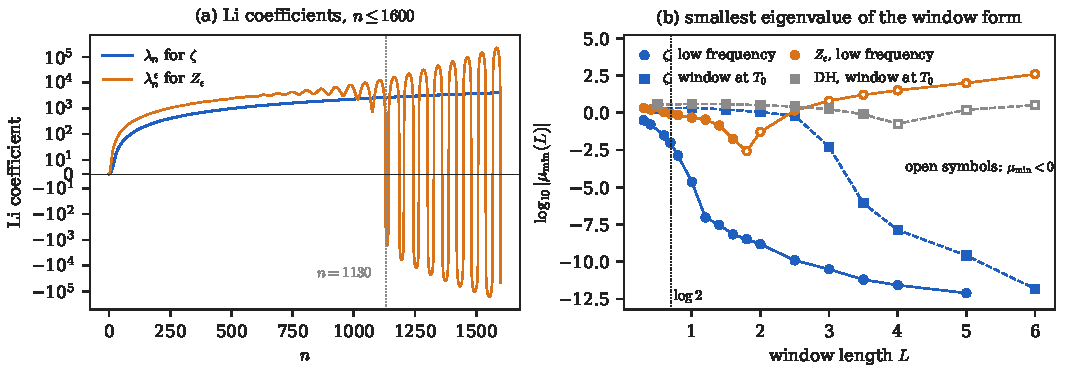
\includegraphics[width=\textwidth]{fig2_comparison.pdf}
\caption{(a) Li coefficients of $\zeta$ and of $Z_\epsilon$ for $n\le1600$ (symmetric logarithmic scale). Those of $Z_\epsilon$ oscillate with growth $1.00735^n$ from the mirror of the zero $s_0$ and are first negative at $n=1130$. (b) The smallest eigenvalue $\mu$ of Weil's form on spline spaces of window length $L$ (knot spacing $0.1$): $\zeta$ and $Z_\epsilon$ at low frequency, $\zeta$ and the Davenport--Heilbronn function near height $T_0=85.699$. Filled symbols are positive values and open symbols negative ones; the dotted line is $L=\log2$.}\label{fig:compare}
\end{figure}

\section{Methods of computation}\label{sec:methods}

\paragraph{Arithmetic.} All computations except the sieve use IEEE double precision (about $16$ significant digits), adaptive Gauss--Kronrod quadrature with relative tolerance $10^{-10}$ to $10^{-13}$, and the trapezoidal rule for integrands that are analytic in a strip, which converges geometrically. The sieve to $10^{10}$ is exact integer arithmetic, segmented in blocks, with $\psi$ and $\theta$ accumulated in double precision.

\paragraph{The functions.} $\zeta(s)$, $\zeta'(s)$ and the Hurwitz function $\zeta(s,\alpha)$ with its derivative are computed by Euler--Maclaurin summation with $\max(60,|s|/\pi+40)$ terms and $20$ to $30$ Bernoulli corrections, the Bernoulli numbers exact as rationals. Dirichlet $L$-functions are combinations of Hurwitz values; $Z_\epsilon$ is computed from the genus identity for $\Re s<4$ and from its Dirichlet series with the exact $r_\epsilon(n)$, $n\le2\times10^5$, for $\Re s\ge4$, and agrees with the lattice sum over $|m|,|n|\le400$ at $s=2.5$ and $3$. The functional equations of $\xi$, $\xi_\epsilon$ and $F_{\mathrm{DH}}$ hold to $7.5\times10^{-15}$ relative at $s=0.3+7.7i$; $\zeta(2)-\pi^2/6=2\times10^{-16}$; and $v(x,0)=0$ off the zeros holds to $10^{-13}$ for $x\le120$, $2\times10^{-8}$ at $x=7005$ and $2\times10^{-7}$ at $x=17143$. The Gamma and digamma functions at complex argument are evaluated by recurrence and the Stirling series. $\Xi_T$, $\Xi_\epsilon$ and their derivatives are computed from the kernel integrals by the trapezoidal rule on $[0,3.5]$ and $[0,8]$, as in \cite{S01}.

\paragraph{Zeros.} The zeros of $\zeta$ on the line below $3000$ ($2469$ of them) are located by Brent's method on sign changes of Hardy's $Z$ on a grid of $1/12$ of the mean spacing, and refined by Newton's method on $\xi$; $\gamma_1=14.134725141734696$ agrees with Odlyzko's table \cite{Odlyzko} to $3\times10^{-15}$. The zeros of $\xi_\epsilon$, $F_{\mathrm{DH}}$, $\Xi+it\Xi'$ and of the heat-flowed functions are located by Newton's method from grid minima, and counted by the argument principle on rectangles.

\paragraph{The flow and the surgery.} $v$ and $u$ are computed from $\xi'/\xi$. The sets $\{v<0\}$ are found on rectangular grids of $3\times10^{-3}$ to $10^{-2}$ in each direction. The Poisson integrals of \cref{thm:jensen} are computed by adaptive quadrature on $|t-x_0|\le12$ with the Green sums over the zeros in that range. The surgery quantities use the closed form of $R$.

\paragraph{Li coefficients and Weil windows.} The coefficients of $F'(w)=\xi'/\xi(1/(1-w))(1-w)^{-2}$ are computed by the discrete Cauchy integral on $|w|=r$ with $M$ equally spaced nodes (fast Fourier transform), $(r,M)=(0.99,8192)$ and $(0.9998,2^{18})$ for $\zeta$ and $(0.975,16384)$, $(0.99,16384)$ for $\xi_\epsilon$, whose coefficients agree to $0.07$ at $n=1130$; the imaginary parts, zero in exact arithmetic, are below $8.2\times10^{-7}$ for $\zeta$ ($n\le30000$) and $8.1\times10^{-9}$ for $\xi_\epsilon$ ($n\le1200$, $r=0.99$). The Weil form is computed from the contour integral of \cref{sec:weil} by the trapezoidal rule with step $0.1$ on $0\le t\le1500$, at $c=1.5$ and $2.6$ for $\zeta$ and $c=2.6$ and $3.2$ for $\xi_\epsilon$ and $F_{\mathrm{DH}}$ (beyond all their zeros), and $\mu(V)$ from the generalised eigenvalue problem with the $L^2$ Gram matrix of the basis. The Lee--Yang sums $S_m$ are computed from the Taylor coefficients of $\log\Xi(-ih)$ by a discrete Cauchy integral with $512$ nodes on $|h|=10$ ($\zeta$) and $|h|=4$ ($\xi_\epsilon$), inside the first zeros $14.13$ and $5.131$.

\paragraph{The heat flow and the spins.} $\Xi_T$ and its derivatives are computed from the kernel integral; the landing time is found by following the zero by Newton's method in $T$; the backward collision times of the Lehmer pairs by locating the change of sign of the local extremum of $\Xi_T$ between the two zeros. On $|z|=1$, $Z_{n,T}(e^{i\vartheta})=P(\cos\vartheta)$ with $P$ a real polynomial of degree $n$, so all $2n$ zeros lie on the circle exactly when $P$ has $n$ zeros in $[-1,1]$; these are counted by Sturm sequences in $80$-digit decimal arithmetic, and $\Lambda_n(K)$ is located by bisection in $T$ after a scan of step $10^{-3}$ downward from $T=0$.

\section{Concluding remarks}\label{sec:concl}
We have shown that the sizes of $\log|\Xi|$ and its gradient on $\Re s\ge1$, known to a tolerance $C_1/\log^2(|x|+2)$, together with the verified zeros, the zero-free region and the zero count, do not decide the sign of the current in $\mathcal U$, and we have given six equivalent forms of \cref{conj:1}: a single-point Jensen--Riesz defect, the Krein--Langer index of the current, the absence of multiple real zeros of the heat flow on $(0,0.2]$, Weil positivity on the Poisson family, the Li radius and a Hausdorff moment property. Unconditionally, the downdraft has measure $\ll T/\log T$ in $[T,2T]$ and touches the zeros off the line, Ford's region carries the updraft, and $\lambda_n>0$ for $n\le10^{12}$. The Epstein and Davenport--Heilbronn functions satisfy the structural statements of \cref{prop:shared} and differ from $\zeta$ in the Euler product and in the properties of \cref{tab:compare}. \Cref{conj:1} is the remaining step; by \cref{mt:surgery} a proof of it must use the arithmetic of $\zeta$ exactly, not through estimates on $\Re s\ge1$, and the comparison functions single out the Euler product as the arithmetic property that separates $\zeta$ from them.

\paragraph{Outlook.} The Euler factors are Lee--Yang polynomials in $\ell^{-s}$ with their zeros on $\Re s=0$, and the next step is to transport this positivity across the strip, through the merge of copies or the heat flow, in a form that the Epstein and Davenport--Heilbronn functions fail. The index formula of \cref{mt:index} and the window forms of \cref{sec:weil} give finite-dimensional quantities on which such a transport can be measured.

\section{Data and sources}\label{sec:data}
\paragraph{External inputs.} All inputs are mathematical; no measured data are used.
\begin{enumerate}[label=(\roman*)]
\item All nontrivial zeros of $\zeta$ with $0<\gamma\le3\cdot10^{12}$ lie on the critical line, and $\Lambda\le0.2$ \cite{PT}; $\Lambda\ge0$ \cite{RT}.
\item Zero-free regions: $\sigma\ge1-1/(5.573412\log|t|)$, $|t|\ge2$ \cite{MT}; $1-\sigma\le1/(57.54(\log|t|)^{2/3}(\log\log|t|)^{1/3})$, $|t|\ge3$ \cite[Thm.~5]{Ford}.
\item $|N(T)-\frac T{2\pi}\log\frac T{2\pi e}-\frac78|\le0.112\log T+0.278\log\log T+2.510+0.2/T$ for $T\ge e$ \cite{Trudgian}.
\item Selberg's density theorem $N(\sigma,T)\ll T^{1-(\sigma-1/2)/4}\log T$ \cite{Selberg46} and Selberg's positive proportion of zeros on the line in intervals \cite[Ch.~X]{Titchmarsh}.
\item The uniform bound on the real parts of the non-real zeros of the heat-flowed function, Theorem~1.5(i) of \cite{Polymath}, and the simplicity of the zeros for $T>\Lambda$ \cite[Cor.~1]{CSV}.
\item Schoenfeld's bound $|\psi(x)-x|<\sqrt x\log^2x/8\pi$, $x\ge73.2$, under RH \cite{Schoenfeld}.
\item Published values used for comparison: $\pi(10^{10})=455{,}052{,}511$ \cite{OEISpi}; $M(10^{10})=-33{,}722$ \cite{OEISM}; $L(10^{10})=-116{,}026$ \cite{OEISL}; the least $x>1$ with $L(x)>0$, $906{,}150{,}257$ \cite{Tanaka}; $\gamma_1$ \cite{Odlyzko}; Spira's zeros of the Davenport--Heilbronn function \cite{Spira}; the values $-5.389\times10^{-69}$ and $-1.31957\times10^{-4}$ of Conrey and Li \cite{CL}.
\item The zero $s_0$ of $Z_\epsilon$, the kernels $\Phi$ and $\Phi_\epsilon$ and the Macdonald expansion are from \cite{S01}.
\end{enumerate}
\paragraph{Computed quantities.} Every other number in the paper is computed from formulas stated in the text by the methods of \cref{sec:methods}: the zeros of $\zeta$ below $3000$, the Lehmer pairs and the zeros of $\xi_\epsilon$ and of $\Xi+it\Xi'$; the flow fields, the Jensen--Riesz defects and the surgery quantities; the Li coefficients of $\zeta$ and $Z_\epsilon$; the Weil window eigenvalues; the $\nu$-flow velocities; the truncation zeros; the de Branges statistics; the heat-flow landing and collision times; the spin-chain constants; the Lee--Yang sums and Hankel determinants; the Tur\'an margins, $V'''$ and $(\log Z)'''$; $r_\epsilon(n)$ for $n\le4\cdot10^5$; and the sieve data to $10^{10}$.

\paragraph{Contributions and use of AI.} The ideas, the research questions, the framework that links the fields, the choice of problems and the direction at every stage are the author's. The derivations, proofs, numerical checks, reference checks and drafting were produced with an AI system working under that direction, and were checked by separate AI review passes. Errors in that material are errors of the AI system, and any found will be corrected in a revised version. Publication-ethics policy (COPE, \emph{Authorship and AI tools}, 2023) does not allow an AI system to be listed as an author, so its use is declared here instead.

\begin{thebibliography}{99}\small
\bibitem{BSY} M.~Balazard, E.~Saias, M.~Yor, Notes sur la fonction $\zeta$ de Riemann, 2, \emph{Adv. Math.} 143 (1999) 284--287.
\bibitem{BerryKeating} M.~V.~Berry, J.~P.~Keating, The Riemann zeros and eigenvalue asymptotics, \emph{SIAM Rev.} 41 (1999) 236--266.
\bibitem{BPY} P.~Biane, J.~Pitman, M.~Yor, Probability laws related to the Jacobi theta and Riemann zeta functions, and Brownian excursions, \emph{Bull. Amer. Math. Soc.} 38 (2001) 435--465.
\bibitem{Bombieri} E.~Bombieri, Remarks on Weil's quadratic functional in the theory of prime numbers, I, \emph{Rend. Mat. Acc. Lincei} (9) 11 (2000) 183--233.
\bibitem{BL} E.~Bombieri, J.~C.~Lagarias, Complements to Li's criterion for the Riemann hypothesis, \emph{J. Number Theory} 77 (1999) 274--287.
\bibitem{BDR} F.~Broucke, G.~Debruyne, S.~Gy.~R\'ev\'esz, Some examples of well-behaved Beurling number systems, \emph{Trans. Amer. Math. Soc.} 378 (2025) 477--501.
\bibitem{Cartwright} N.~D.~Cartwright, A non-negative Wigner-type distribution, \emph{Physica A} 83 (1976) 210.
\bibitem{CC} A.~Connes, C.~Consani, Weil positivity and trace formula, the archimedean place, \emph{Selecta Math. (N.S.)} 27 (2021) 77.
\bibitem{CL} J.~B.~Conrey, X.-J.~Li, A note on some positivity conditions related to zeta and $L$-functions, \emph{Int. Math. Res. Notices} 2000, no.~18, 929--940.
\bibitem{CNV} G.~Csordas, T.~S.~Norfolk, R.~S.~Varga, The Riemann hypothesis and the Tur\'an inequalities, \emph{Trans. Amer. Math. Soc.} 296 (1986) 521--541.
\bibitem{CSV} G.~Csordas, W.~Smith, R.~S.~Varga, Lehmer pairs of zeros, the de Bruijn--Newman constant $\Lambda$, and the Riemann hypothesis, \emph{Constr. Approx.} 10 (1994) 107--129.
\bibitem{DH} H.~Davenport, H.~Heilbronn, On the zeros of certain Dirichlet series I, II, \emph{J. London Math. Soc.} 11 (1936) 181--185, 307--312.
\bibitem{deBrangesBook} L.~de Branges, \emph{Hilbert Spaces of Entire Functions}, Prentice-Hall, Englewood Cliffs, NJ, 1968.
\bibitem{deBranges86} L.~de Branges, The Riemann hypothesis for Hilbert spaces of entire functions, \emph{Bull. Amer. Math. Soc. (N.S.)} 15 (1986) 1--17.
\bibitem{deBruijn} N.~G.~de Bruijn, The roots of trigonometric integrals, \emph{Duke Math. J.} 17 (1950) 197--226.
\bibitem{Ford} K.~Ford, Zero-free regions for the Riemann zeta function, in \emph{Number Theory for the Millennium II} (Urbana, IL, 2000), A K Peters, Natick, MA, 2002, 25--56.
\bibitem{Griffiths69} R.~B.~Griffiths, Rigorous results for Ising ferromagnets of arbitrary spin, \emph{J. Math. Phys.} 10 (1969) 1559--1565.
\bibitem{Hausdorff} F.~Hausdorff, Summationsmethoden und Momentfolgen. I, \emph{Math. Z.} 9 (1921) 74--109.
\bibitem{Hilberdink} T.~W.~Hilberdink, Well-behaved Beurling primes and integers, \emph{J. Number Theory} 112 (2005) 332--344.
\bibitem{KK} J.~Kaczorowski, M.~Kulas, On the non-trivial zeros off the critical line for $L$-functions from the extended Selberg class, \emph{Monatsh. Math.} 150 (2007) 217--232.
\bibitem{KW} M.~Kaltenb\"ack, H.~Woracek, Pontryagin spaces of entire functions I, \emph{Integral Equations Operator Theory} 33 (1999) 34--97.
\bibitem{Keiper} J.~B.~Keiper, Power series expansions of Riemann's $\xi$ function, \emph{Math. Comp.} 58 (1992) 765--773.
\bibitem{KKL} H.~Ki, Y.-O.~Kim, J.~Lee, On the de Bruijn--Newman constant, \emph{Adv. Math.} 222 (2009) 281--306.
\bibitem{KL} M.~G.~Krein, H.~Langer, \"Uber einige Fortsetzungsprobleme, die eng mit der Theorie hermitescher Operatoren im Raume $\Pi_\kappa$ zusammenh\"angen. I. Einige Funktionenklassen und ihre Darstellungen, \emph{Math. Nachr.} 77 (1977) 187--236.
\bibitem{Lagarias99} J.~C.~Lagarias, On a positivity property of the Riemann $\xi$-function, \emph{Acta Arith.} 89 (1999) 217--234; correction, \emph{Acta Arith.} 116 (2005) 293--294.
\bibitem{Lagarias05} J.~C.~Lagarias, Zero spacing distributions for differenced $L$-functions, \emph{Acta Arith.} 120 (2005) 159--184.
\bibitem{LeeYang} T.~D.~Lee, C.~N.~Yang, Statistical theory of equations of state and phase transitions. II. Lattice gas and Ising model, \emph{Phys. Rev.} 87 (1952) 410--419.
\bibitem{Li} X.-J.~Li, The positivity of a sequence of numbers and the Riemann hypothesis, \emph{J. Number Theory} 65 (1997) 325--333.
\bibitem{MT} M.~J.~Mossinghoff, T.~S.~Trudgian, Nonnegative trigonometric polynomials and a zero-free region for the Riemann zeta-function, \emph{J. Number Theory} 157 (2015) 329--349.
\bibitem{Newman74} C.~M.~Newman, Zeros of the partition function for generalized Ising systems, \emph{Comm. Pure Appl. Math.} 27 (1974) 143--159.
\bibitem{Newman76} C.~M.~Newman, Fourier transforms with only real zeros, \emph{Proc. Amer. Math. Soc.} 61 (1976) 245--251.
\bibitem{Newman91} C.~M.~Newman, The GHS inequality and the Riemann hypothesis, \emph{Constr. Approx.} 7 (1991) 389--399.
\bibitem{Odlyzko} A.~M.~Odlyzko, Tables of zeros of the Riemann zeta function, \url{https://www-users.cse.umn.edu/~odlyzko/zeta_tables/index.html} (accessed 25 September 2026).
\bibitem{OEISpi} OEIS Foundation, Sequence A006880, number of primes $<10^n$, \emph{The On-Line Encyclopedia of Integer Sequences}, \url{https://oeis.org/A006880} (accessed 25 September 2026).
\bibitem{OEISM} OEIS Foundation, Sequence A084237, $a(n)=M(10^n)$, where $M(n)$ is Mertens's function, \emph{The On-Line Encyclopedia of Integer Sequences}, \url{https://oeis.org/A084237} (accessed 25 September 2026).
\bibitem{OEISL} OEIS Foundation, Sequence A090410, values of $L(10^n)$, where $L(n)$ is the summatory function of the Liouville function, \emph{The On-Line Encyclopedia of Integer Sequences}, \url{https://oeis.org/A090410} (accessed 25 September 2026).
\bibitem{PT} D.~Platt, T.~Trudgian, The Riemann hypothesis is true up to $3\cdot10^{12}$, \emph{Bull. London Math. Soc.} 53 (2021) 792--797.
\bibitem{Polya26} G.~P\'olya, Bemerkung \"uber die Integraldarstellung der Riemannschen $\xi$-Funktion, \emph{Acta Math.} 48 (1926) 305--317.
\bibitem{Polymath} D.~H.~J.~Polymath, Effective approximation of heat flow evolution of the Riemann $\xi$ function, and a new upper bound for the de Bruijn--Newman constant, \emph{Res. Math. Sci.} 6 (2019) 31.
\bibitem{Ransford} T.~Ransford, \emph{Potential Theory in the Complex Plane}, London Mathematical Society Student Texts 28, Cambridge University Press, Cambridge, 1995.
\bibitem{RT} B.~Rodgers, T.~Tao, The de Bruijn--Newman constant is non-negative, \emph{Forum Math. Pi} 8 (2020) e6.
\bibitem{Schoenfeld} L.~Schoenfeld, Sharper bounds for the Chebyshev functions $\theta(x)$ and $\psi(x)$. II, \emph{Math. Comp.} 30 (1976) 337--360.
\bibitem{Selberg46} A.~Selberg, Contributions to the theory of the Riemann zeta-function, \emph{Arch. Math. Naturvid.} 48 (1946) 89--155.
\bibitem{S01} A.~Singh, Pair Balance and the Riemann Zeros: The Signed Current, the Mirror and the Merge, and the Prime Two, manuscript, 25 September 2026.
\bibitem{S02} A.~Singh, The Reversible Half and the Third Body: Pairs and Triads in Measurement Records and the Three-Body Problem, manuscript, 25 September 2026.
\bibitem{S03} A.~Singh, The Riemann Kernel as a Quantum State: Wigner Negativity, Decoherence at the Thirds and Lee--Yang Zeros, manuscript, 25 September 2026.
\bibitem{S04} A.~Singh, Which Member Carries: Two-State Pairs from Atoms to Gas Sensors, and D\"obereiner's Triads as Balanced Pairs, manuscript, 25 September 2026.
\bibitem{S05} A.~Singh, The Balanced Pair in Excitable Tissue: What a Membrane Reading Determines, and the Balanced Cortex, manuscript, 25 September 2026.
\bibitem{S06} A.~Singh, Three Is Enough: Radix Economy, Balanced-Ternary Arithmetic and Ternary-Weight Networks, manuscript, 25 September 2026.
\bibitem{S07} A.~Singh, The Four Giants as Balanced Pairs: Throats, Hearts, the Gas Ladder and the Interstellar Visitors, manuscript, 25 September 2026.
\bibitem{S08} A.~Singh, What a Zero Is: One Involution across Mathematics, Physics, Chemistry, Neuroscience, Computation and the Giant Planets, manuscript, 25 September 2026.
\bibitem{SD} J.~Sondow, C.~Dumitrescu, A monotonicity property of Riemann's xi function and a reformulation of the Riemann hypothesis, \emph{Period. Math. Hungar.} 60 (2010) 37--40.
\bibitem{Spira} R.~Spira, Some zeros of the Titchmarsh counterexample, \emph{Math. Comp.} 63 (1994) 747--748.
\bibitem{Tanaka} M.~Tanaka, A numerical investigation on cumulative sum of the Liouville function, \emph{Tokyo J. Math.} 3 (1980) 187--189.
\bibitem{Titchmarsh} E.~C.~Titchmarsh, \emph{The Theory of the Riemann Zeta-Function}, 2nd ed., revised by D.~R.~Heath-Brown, Oxford University Press, Oxford, 1986.
\bibitem{Trudgian} T.~S.~Trudgian, An improved upper bound for the argument of the Riemann zeta-function on the critical line II, \emph{J. Number Theory} 134 (2014) 280--292.
\bibitem{Weil} A.~Weil, Sur les ``formules explicites'' de la th\'eorie des nombres premiers, \emph{Comm. S\'em. Math. Univ. Lund}, tome suppl\'ementaire (1952) 252--265.
\end{thebibliography}
\end{document}
